\documentclass{article}
\usepackage[english]{babel}
\usepackage[a4,top=2cm,bottom=2cm,left=3cm,right=3cm,marginparwidth=1.75cm]{geometry}
\usepackage{amsmath}
\usepackage{graphicx}
\usepackage[colorlinks=true, allcolors=blue]{hyperref}

\title{Project 1: Inference of BK initial condition}
\author{Carlisle Aurabelle Casuga}

\begin{document}
\maketitle

\section{MV}

For the initial run on the MV model with 50 design points, sampled using plain latin hypercube sampling within a wide parameter  space with bounds: $Q_{s0}²$ = [0.001, 2.0] 1/GeV²; $C²$ = [0.1, 100.0], and $\sigma_{0}/2$ = [1.0, 40.0] mb, the following results were obtained: 

\begin{figure}[h]
\centering
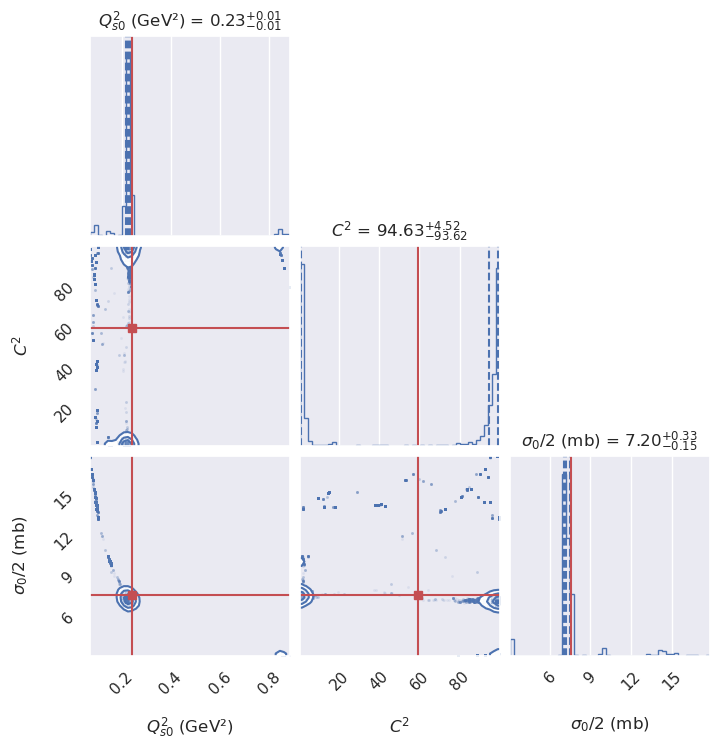
\includegraphics[width=0.5\textwidth]{figs\mv_50d_initial_50w.png}
\caption{Initial run on the MV model with 50 design points}
\label{fig:mv_50d_50w}
\end{figure}

Figure \ref{fig:mv_50_1} is sampled with 50 walkers, total 1500 steps, 500 of which are burn steps. This will provide us with a rough estimate of the posterior distribution of the parameters. Actual values of the parameters at the 16\%, 50\%, and 84\% percentiles are:

$Q_{s0}²$: [(0.16, 0.21728015544863194), (0.5, 0.2275510190337838), (0.84, 0.23450182482460977)]
$C²$: [(0.16, 1.0035763833397198), (0.5, 94.62810202727259), (0.84, 99.14833702805878)]
$\sigma_{0}/2$: [(0.16, 7.052807276014379), (0.5, 7.200058879152208), (0.84, 7.5276927226268135)]

From the 2013 paper, the values of the parameters are: $Q_{s0}²$ = 0.104 GeV²; $C²$ = 14.5, and $\sigma_{0}/2$ = 18.2 mb. We have a large disparity between these values and the values we obtained from the initial run. Next run we can tighten the bounds of $Q_{s0}²$ = [0.001, 0.5] but widen the C² parameters to [0.05, 150.0] to accomodate the peak at large values of C².

We show here the chain of walkers in this run where some of the walkers are stuck in areas of low likelihood. To resolve this, we  double the number of walkers to 100 and run the sampler for 1000 burn steps. Then we (emcee) sample within a tighter space surrounding the posterior distribution peaks. 

\begin{figure}[h]
\centering
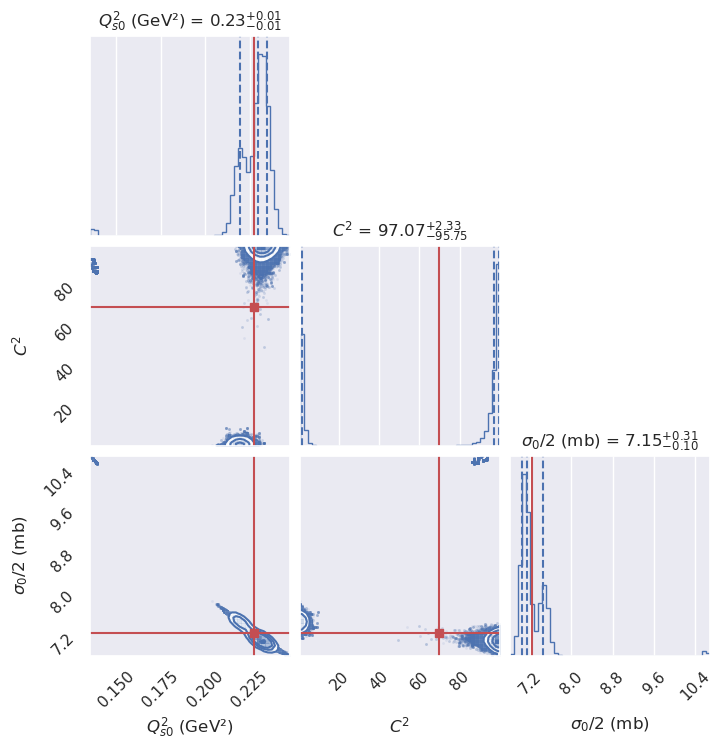
\includegraphics[width=0.5\textwidth]{figs\mv_50d_initial_100w.png}
\caption{Same MV run but with 100 walkers}
\label{fig:mv_50d_100w}
\end{figure}

\section{MVe adventures}

With the MVe model, there are 4 free model parameters to be fitted against: $$Q_{s0}²$$ $$C²$$ $$\sigma_{0}/2$$ with the addition of $$e_c$$. The bounds of the LHS sampling of the parameters are: $Q_{s0}²$ = [0.001, 2.0] 1/GeV²; $C²$ = [0.1, 100.0], and $\sigma_{0}/2$ = [1.0, 40.0] mb. The bounds of $e_c$ are [0.5, 100.0]. In this run we aimed to sample 49 design points through both plain LHS and orthogonal LHS. In both cases the GPE performed very poorly with very large errors and off predictions. The next run is to try with more design points, specifically 121 design points.

The GPE is ran with an RBF + WhiteKernel kernels and whose initial hyperparameters were set at "length_scale = 1 * np.ones(theta.shape[1]), length_scale_bounds = (1e-10, 1e10)" but with the Whitekernel with default parameters. We also set n_restart_optimizer = 2 so that a better fit is made. With these settings there is no error warning regarding the determination of the optimal hyperparameter of the kernels. With 10\% of the training data as validation data and n=5 principal components, the GPE produces the following predictions for a single kinematical point. We also show  the zscore for a single kinematical point.

\begin{figure}[h]
\centering
\includegraphics[width=0.5\textwidth]{figs\mve_121d_gpe.png}
\caption{GPE predictions for a single kinematical point}
\label{fig:mve_121d_gpe}
\end{figure}

\begin{figure}[h]
\centering
\includegraphics[width=0.5\textwidth]{figs\mve_121d_zscore.png}
\caption{Zscore for a single kinematical point}
\label{fig:mve_121d_zscore}
\end{figure}

The emcee sampling for 100 walkers (30 minutes run time) is performed and from the chain, the walkers were not properly converged as we can see from the chain plot. We run the sampler again for more walkers (500) and less $Q_s0²$ space, in the hopes of finding a better convergence. Unfortunately, we show here that it does converge the walkers but nonetheless a poor sampling distribution is obtained. 

\begin{figure}[h]
\centering
\includegraphics[width=0.5\textwidth]{figs\mve_121d_500w.png}
\caption{MVe run with 500 walkers}
\label{fig:mve_121d_500w}
\end{figure}

with quantile values
Quantiles: [(0.16, 0.10444113262841531), (0.5, 0.1100391634489063), (0.84, 0.16343216074397923)]
Quantiles: [(0.16, 12.423226137980059), (0.5, 65.03766366566634), (0.84, 66.67212300526586)]
Quantiles: [(0.16, 15.868392244095453), (0.5, 48.19438130661283), (0.84, 81.1793240923539)]
Quantiles: [(0.16, 5.978122615546301), (0.5, 6.203794380396528), (0.84, 6.79909337149499)]

To further prove that this is not a good sampling run, the mean acceptance is 0.197. The optimal acceptance ratio is .2 to .5.

I had a suspicion on whether there was something wrong with generating the training set. However, when I tried using the same code to generate the training set for past runs, there was no problems. Let's compare the bayesian sampling in both cases. The first one is the old training set while the second one the new one. There is no difference in the sampling distribution besides the old one just had more samples. So there was no weird change to the training set code.

\begin{figure}[h]
\centering
\includegraphics[width=0.5\textwidth]{figs\4p_new.png}
\caption{tight MVe run with old training set}
\label{fig:4p_new}
\end{figure}

\begin{figure}[h]
\centering
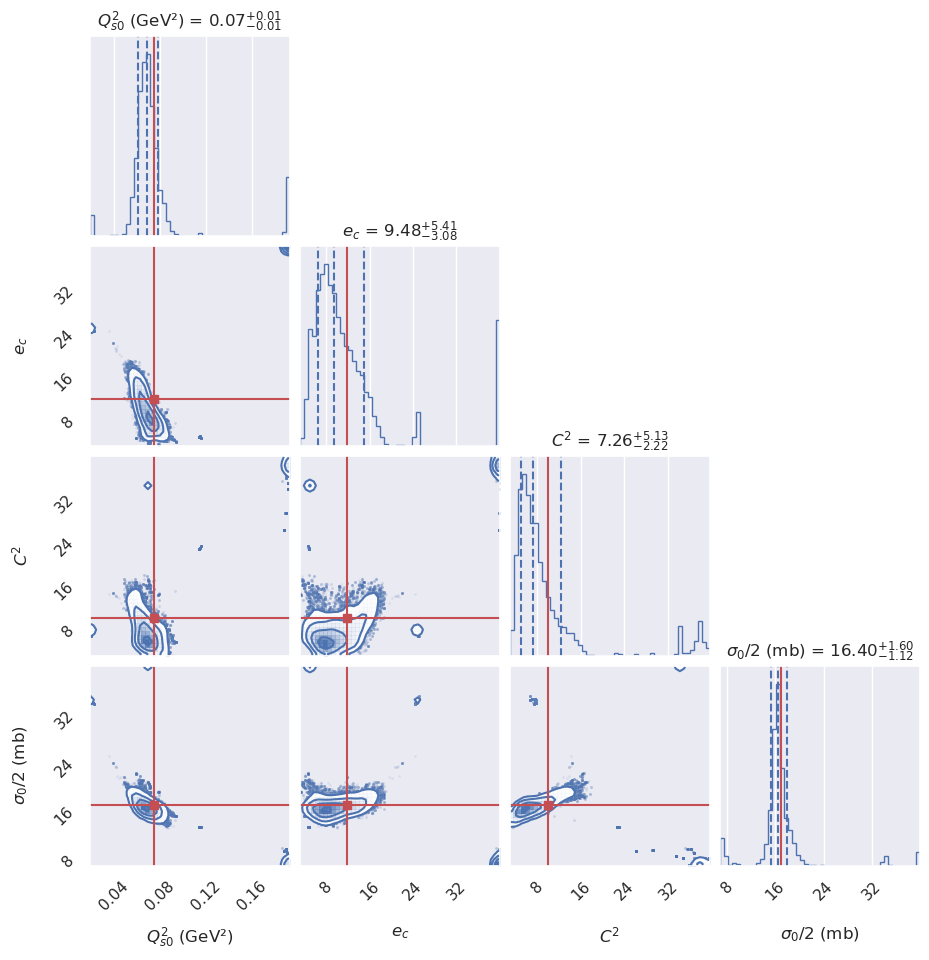
\includegraphics[width=0.5\textwidth]{figs\4p_new_vs.png}
\caption{tight MVe run with new training set}
\label{fig:4p_new_vs}
\end{figure}

I had the idea of combining a past MVe run with this current one. This old run has LH samples within a tighter parameter space where $Q_{s0}²$ = [0.001, 0.2] 1/GeV²; $e_c$ = [0.5, 40.0] ; $C²$ = [0.1, 40.0], and $\sigma_{0}/2$ = [1.0, 40.0] mb. This involved generating a training set from Q² = 2.0 GeV² to 10 GeV² to cover what was lacking in the old run and then combining the two training sets and parameter vector sets. So that a wider array of training data and parameter values (denser in the tighter region) can give us the areas where the likelihood is maximized. (Theta file and training file was appended).

The sampling distribution is shown below. 

Quantiles: [(0.16, 0.06739340877316732), (0.5, 0.11670826980103077), (0.84, 0.21280114410076745)]
Quantiles: [(0.16, 11.079119769318801), (0.5, 60.1650779980113), (0.84, 99.0661828030286)]
Quantiles: [(0.16, 9.1138629738339), (0.5, 14.641110632950689), (0.84, 65.43275805593659)]
Quantiles: [(0.16, 4.765888420339204), (0.5, 6.945807097304044), (0.84, 17.08536031618019)]

\begin{figure}
\centering
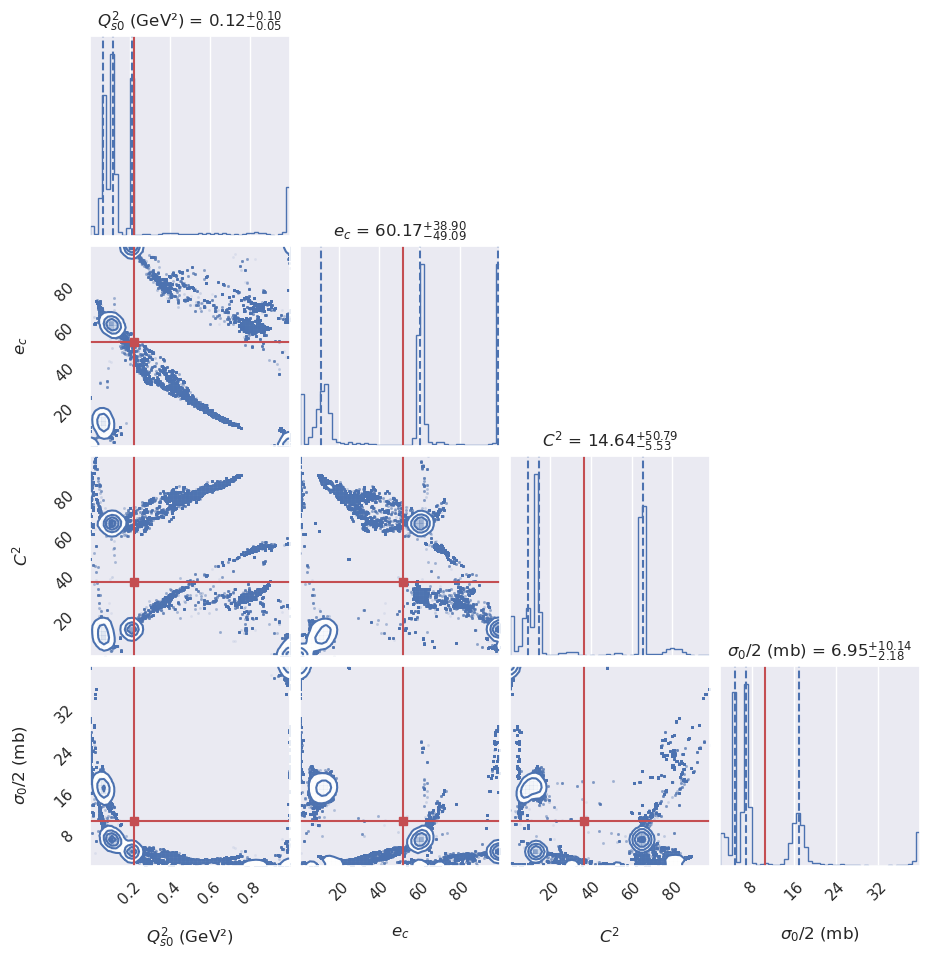
\includegraphics[width=0.5\textwidth]{figs\mve_121+100d_500w.png}
\caption{MVe run with 500 walkers with hybrid training set}
\label{fig:mve_121+100d_500w}
\end{figure}

\begin{figure}
\centering
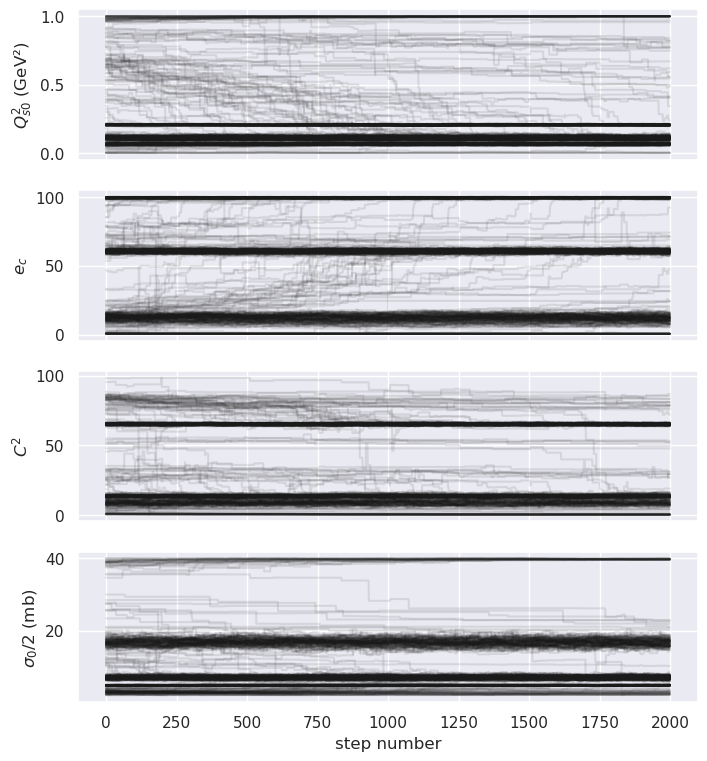
\includegraphics[width=0.5\textwidth]{figs\mve_121+100d_500w_chain.png}
\caption{MVe run with 500 walkers with hybrid training set: chain}
\label{fig:mve_121+100d_500w_chain}
\end{figure}

\begin{figure}
\centering
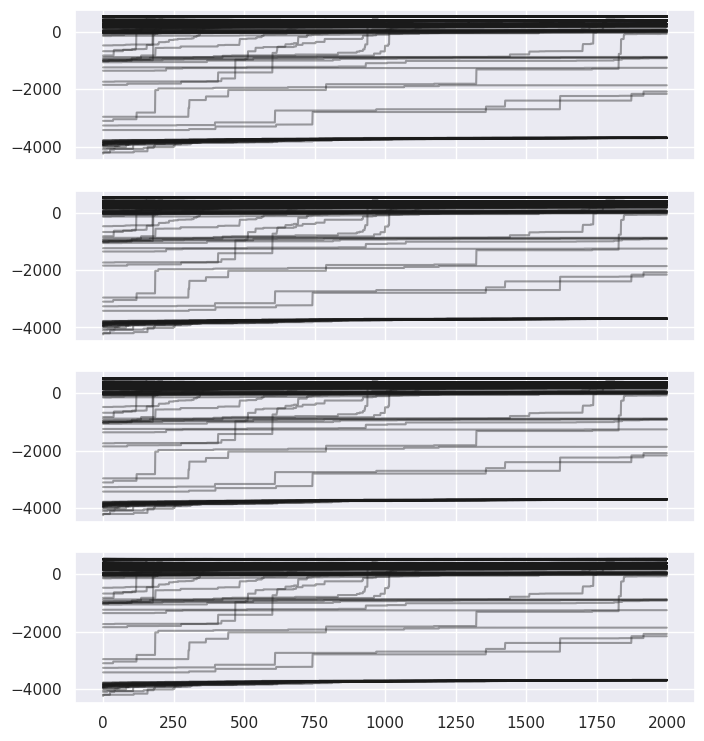
\includegraphics[width=0.5\textwidth]{figs\mve_121+100d_500w_logprob.png}
\caption{MVe run with 500 walkers with hybrid training set: log prob}
\label{fig:mve_121+100d_500w_logprob}
\end{figure}

\begin{figure}
\centering
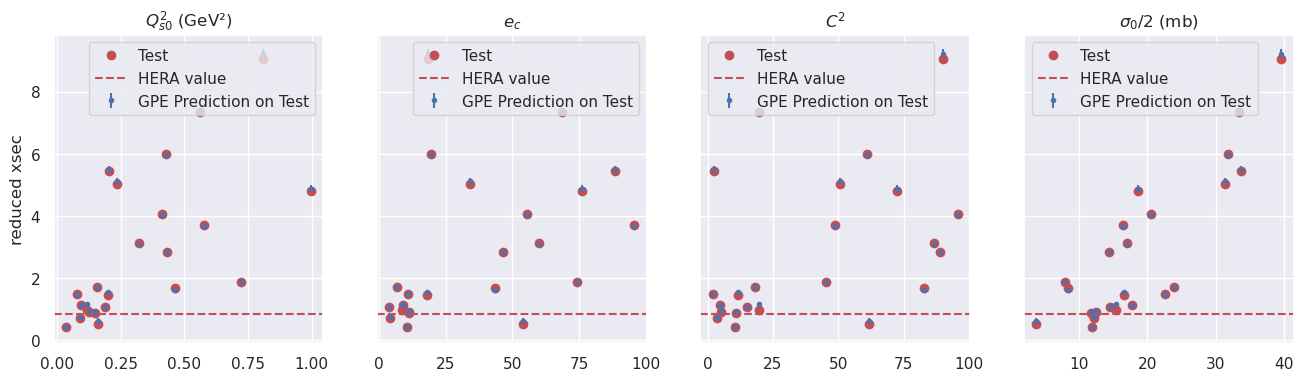
\includegraphics[width=0.5\textwidth]{figs\mve_121+100d_gpe.png}
\caption{GPE prediction at a single kinematical point}
\label{fig:mve_121+100d_gpe}
\end{figure}

Even if the GPE is performing well, because the walkers were initialized in a very large space, they struggle to find the optimal likelihood spots. Despite converegences at localized spots, the log prob chain shows that they settle at different values of posterior probabilities. The 1d and 2d histograms shown are therefore not very reliable. 

Let's try it again with a smaller initialization space and less walkers.

\begin{figure}
\centering
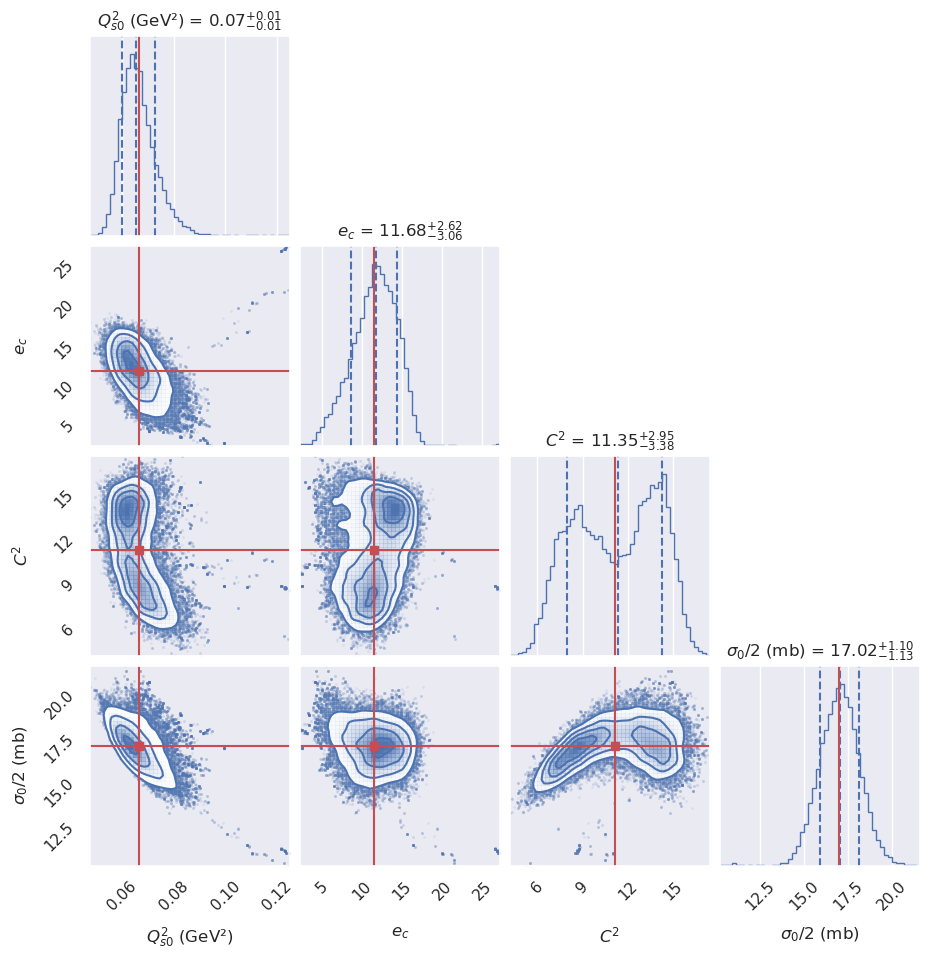
\includegraphics[width=0.5\textwidth]{figs\mve_121+100d_100w_narrow.png}
\caption{MVe run with 100 walkers with hybrid training set}
\label{fig:mve_121+100d_100w_narrow}
\end{figure}

This shows proper convergence in both posterior distributions and sample chain. However, there is no proper peak for the C² posterior distribution. I tried setting a narrower initialization for the other parameters and set C² to be initialized at a wider bound [0.1, 100.0] but that did not help as can be seen below.

\begin{figure}
\centering
\includegraphics[width=0.5\textwidth]{figs\mve_121+100d_100w_narrowinit_wideC2.png}
\caption{MVe run with 100 walkers with hybrid training set: C² initialized at [0.1, 100.0]}
\label{fig:mve_121+100d_100w_narrowinit_wideC2}
\end{figure}

So far we have not been able to constrain C². Next, I have a suspicion that training the gpe for such a wide parameter space messes up the correlations between the values of the reduced cross section. So we switch back to the complete training set but with training set generated with design points sampled in a narrower bound where $Q_{s0}²$ = [0.001, 0.2] 1/GeV²; $e_c$ = [0.5, 40.0] ; $C²$ = [0.1, 40.0], and $\sigma_{0}/2$ = [10.0, 30.0] mb, a more reasonable space centered around the values found in the rcbk paper. 

The GPE was trained for 403 kinematical points where the Q^2 range is from 2.0 to 50.0 GeV^2 where the BK limit is valid. The GPE prediction did very well with 10 percent test data and 6 principal components chosen via qualitative scan of the z-score for different number of components shown below:

\begin{figure}
\centering
\includegraphics[width=0.5\textwidth]{figs\mve_100d_zscore.png}
\caption{Z-score for different number of principal components}
\label{fig:mve_100d_zscore}
\end{figure}

And this is how the GPE performs for a single kinematical point. 

\begin{figure}
\centering
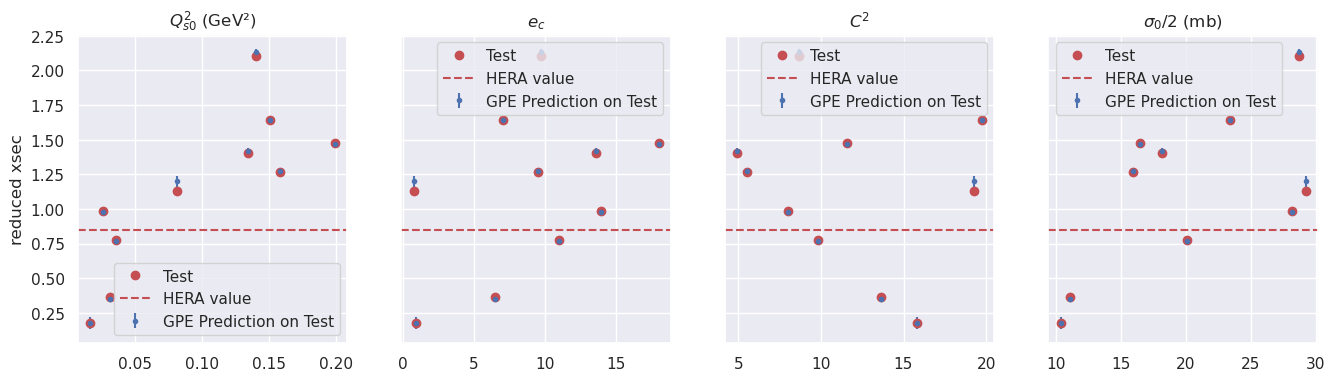
\includegraphics[width=0.5\textwidth]{figs\mve_100d_gpe.png}
\caption{GPE prediction at a single kinematical point}
\label{fig:mve_100d_gpe}
\end{figure}

And this is how the emcee sampling went (using 100 walkers, 2000 burn steps and 1000 production steps):

\begin{figure}
\centering
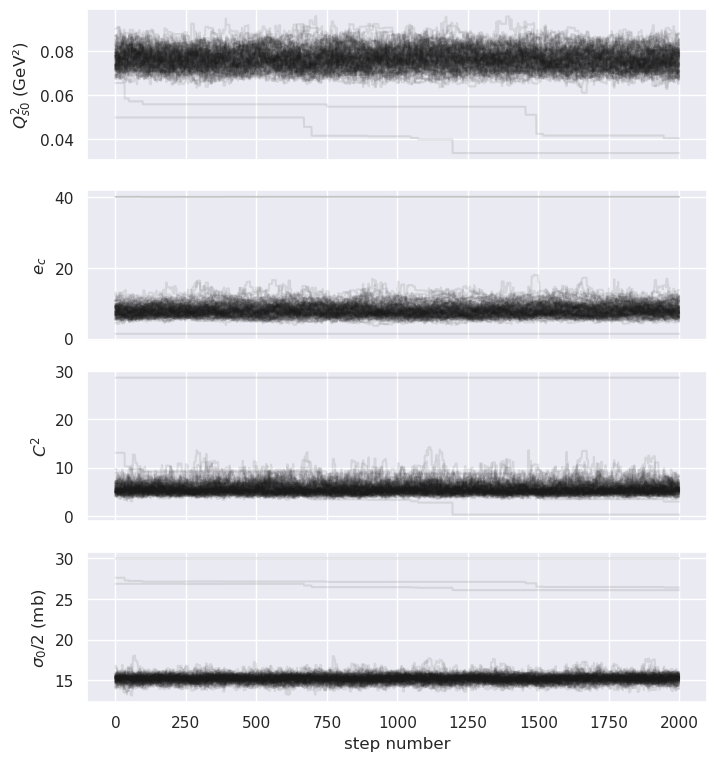
\includegraphics[width=0.5\textwidth]{figs\mve_100d_100w_chain.png}
\caption{MVe run with 100 walkers with design points that have smaller parameter space: chain}
\label{fig:mve_100d_100w_chain}
\end{figure}

\begin{figure}
\centering
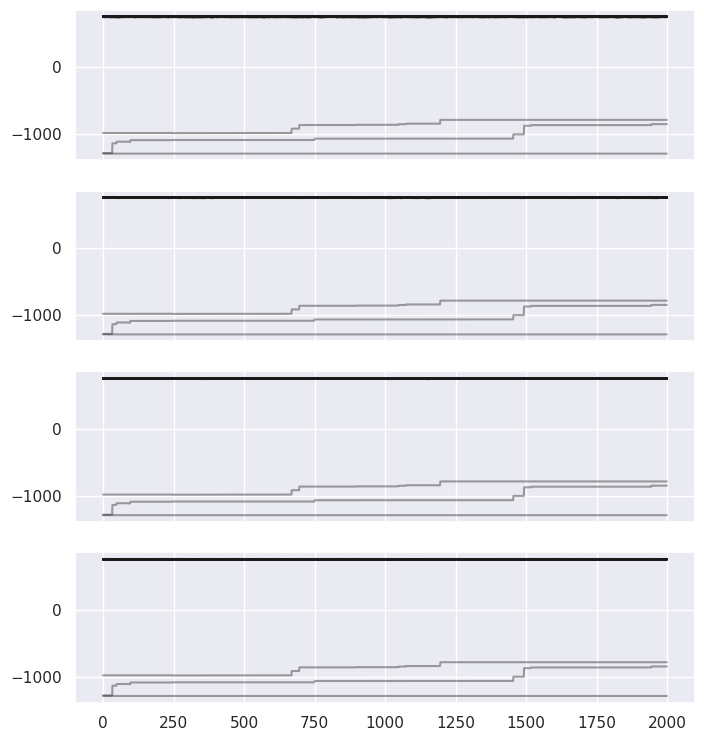
\includegraphics[width=0.5\textwidth]{figs\mve_100d_100w_logprob.png}
\caption{MVe run with 100 walkers with design points that have smaller parameter space: log prob}
\label{fig:mve_100d_100w_logprob}
\end{figure}

\begin{figure}
\centering
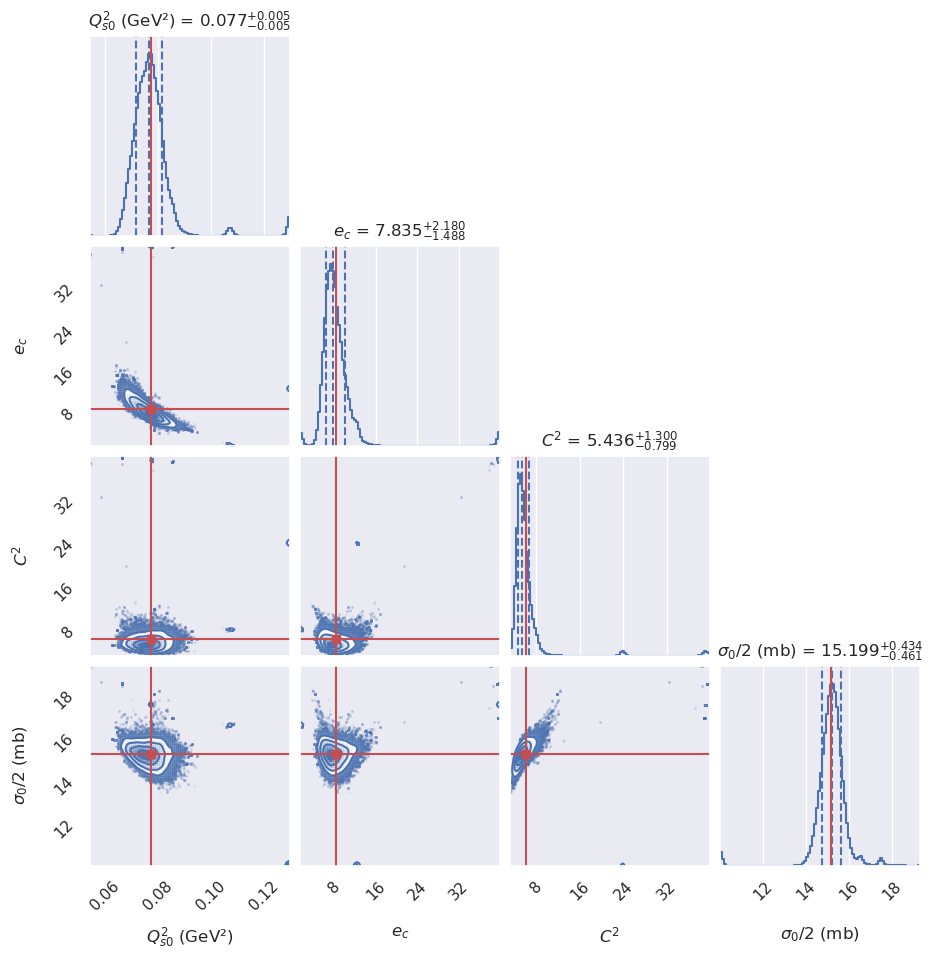
\includegraphics[width=0.5\textwidth]{figs\mve_100d_100w.png}
\caption{MVe run with 100 walkers with design points that have smaller parameter space}
\label{fig:mve_100d_100w}
\end{figure}

As can be seen, this is reliable because the values have converged pretty nicely. These plots have quantile values at:

Quantiles: [(0.16, 0.07167898754863827), (0.5, 0.07659888520137269), (0.84, 0.08143020768290565)]
Quantiles: [(0.16, 6.3469525054075735), (0.5, 7.834631953247264), (0.84, 10.01465421992532)]
Quantiles: [(0.16, 4.636596860991138), (0.5, 5.436055036040134), (0.84, 6.73622171023949)]
Quantiles: [(0.16, 14.737995258738518), (0.5, 15.199272555845912), (0.84, 15.633713579507749)]

Mean and acceptance fraction:
$Q_{s0}^{2}$ (GeV²)= 0.077
$e_c$= 8.417
$C^{2}$= 6.192
$\sigma_0/2$ (mb)= 15.173
Mean acceptance fraction: 0.400

\subsection{Final Training}

To improve the sampling we initialize our walkers in a very narrow portion of the parameter space with the prior knowledge already of what the posterior median peaks are. The bounds of the initialization are l_bounds_in = [0.05, 7.0, 5.0, 14.0] and u_bounds_in = [0.09, 11.0, 7.0, 16.0]. The results converge pretty nicely and make very nice posterior distributions.

\begin{figure}
\centering
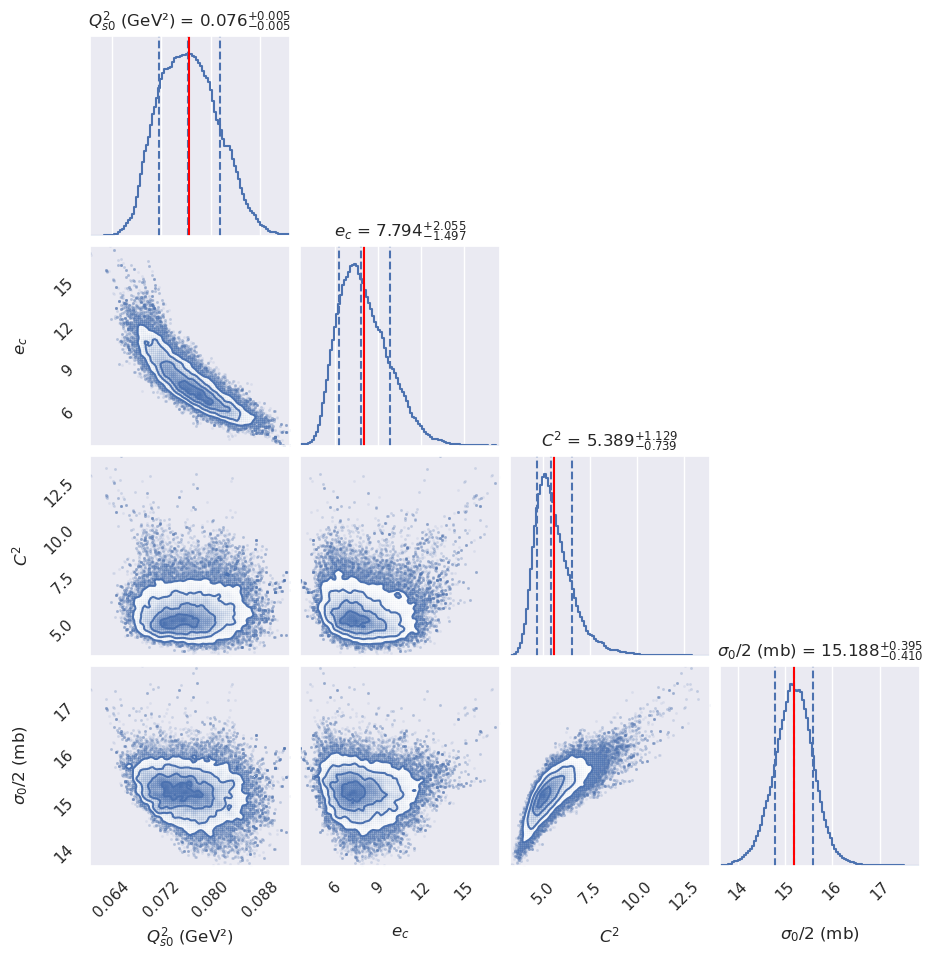
\includegraphics[width=0.5\textwidth]{figs\mve_100d_100w_narrowinit.png}
\caption{MVe run with 100 walkers with design points that have even smaller parameter space}
\label{fig:mve_100d_100w_narrow}
\end{figure}

\begin{figure}
\centering
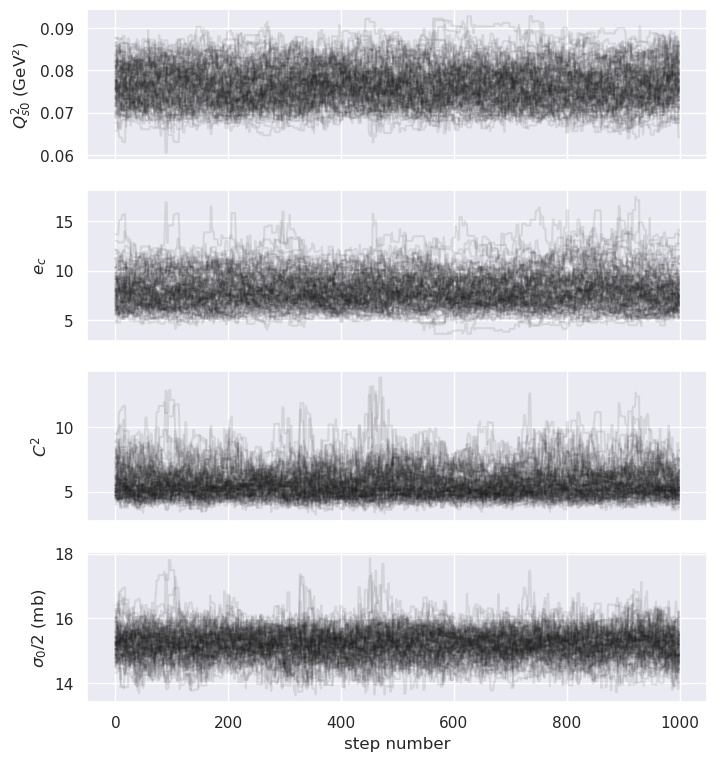
\includegraphics[width=0.5\textwidth]{figs\mve_100d_100w_narrowinit_chain.png}
\caption{MVe run with 100 walkers with design points that have even smaller parameter space: chain}
\label{fig:mve_100d_100w_narrow_chain}
\end{figure}

\begin{figure}
\centering
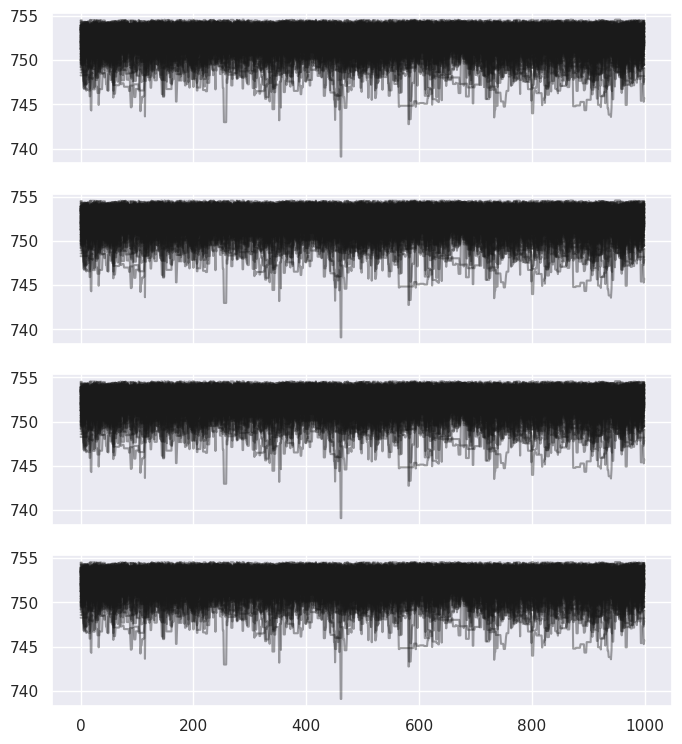
\includegraphics[width=0.5\textwidth]{figs\mve_100d_100w_narrowinit_logprob.png}
\caption{MVe run with 100 walkers with design points that have even smaller parameter space: log prob}
\label{fig:mve_100d_100w_narrow_logprob}
\end{figure}

With mean values:
$Q_{s0}^{2}$ (GeV²)= 0.077
$e_c$= 8.039
$C^{2}$= 5.589
$\sigma_0/2$ (mb)= 15.185
Mean acceptance fraction: 0.418

\subsection{Sampling from the Posterior and MAP estimates}

One hundred parameter vectors are now obtained from these posterior distributions (saved in "mve_100d_100w_sampled_from_posterior.txt" file) and obtained model cross sections from these samples. All parameter samples were saved in "mve/100d_100w_allsamples.txt".

These values are ploted against experimental data. Say, for example, at Q2 = 45.0 GeV and sqrt(s) = 318.0 GeV, we compare the training set vs 100 design points sampled in the posterior.

\begin{figure}
\centering
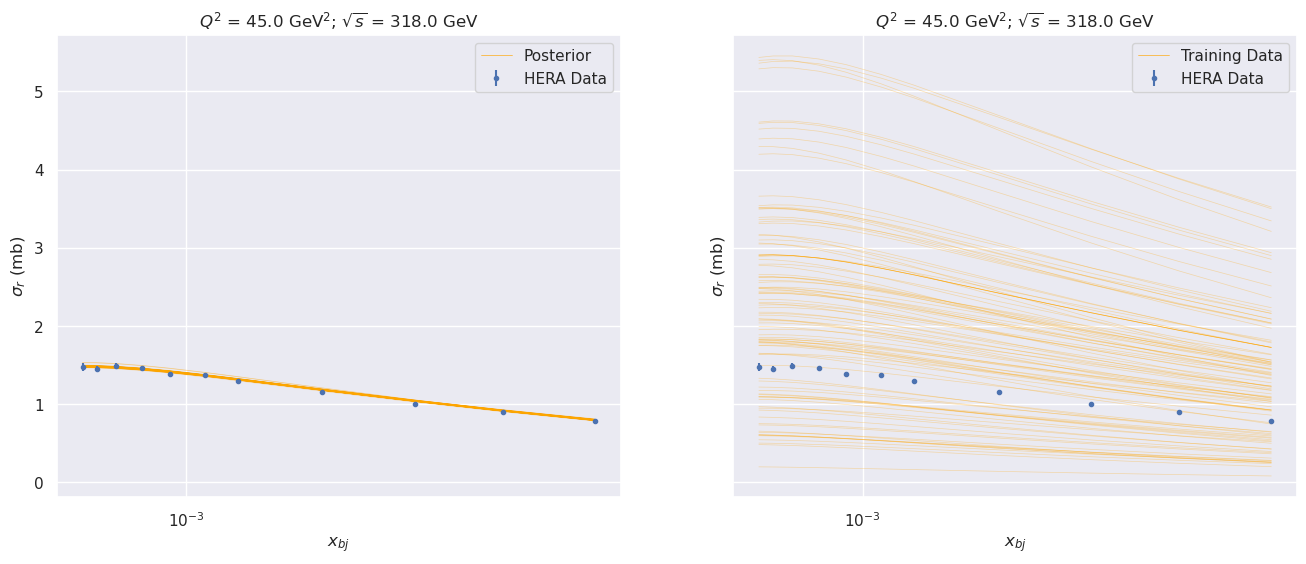
\includegraphics[width=0.5\textwidth]{figs\mve_train_vs_post_45_318.png}
\caption{Training set vs posterior samples at Q2 = 45.0 GeV and sqrt(s) = 318.0 GeV}
\label{fig:mve_train_vs_post_45_318}
\end{figure}

This shows that the samples from the posterior match very well with data, this goes for other values of Q as well.

\begin{figure}
\centering
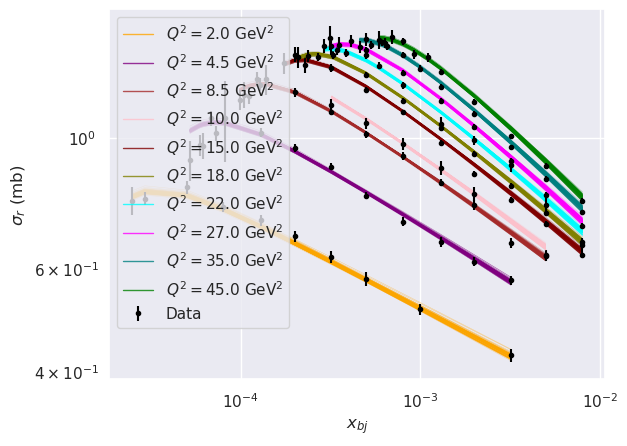
\includegraphics[width=0.5\textwidth]{figs\mve_post_vs_data_manyq2.png}
\caption{Posterior samples vs data at different values of Q2}
\label{fig:mve_post_vs_data_manyq2}
\end{figure}

We then obtain what are called MAP estimates (maximum a posteriori) which are the parameter values that maximize the posterior distribution. Using the scipy minimize function, we minimize the negative of the log posterior function. The MAP estimates are: [ 0.07696357  7.46144896  5.00327994 15.02871265]. These estimates are the ones presented as the "best fit" where the model cross sections match the data the most.

Below we show a plot of the reduced cross sections calculated by the emulator using MAP estimates vs the data and also vs the posterior median where we also show the 68\% confidence interval at kinematical point Q² = 45.0 GeV and sqrt(s) = 318.0 GeV.

\begin{figure}
\centering
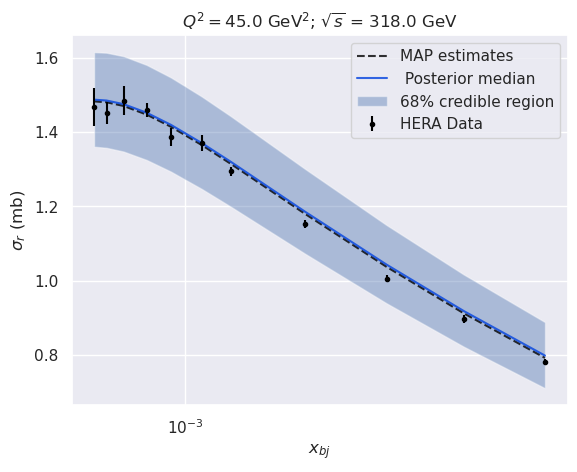
\includegraphics[width=0.5\textwidth]{figs\mve_map_vs_median_45_318.png}
\caption{MAP vs median at Q2 = 45.0 GeV and sqrt(s) = 318.0 GeV}
\label{fig:mve_map_vs_median_45_318}
\end{figure}

Also another one at same Q2 but sqrt(s) = 225.0 GeV.

\begin{figure}
\centering
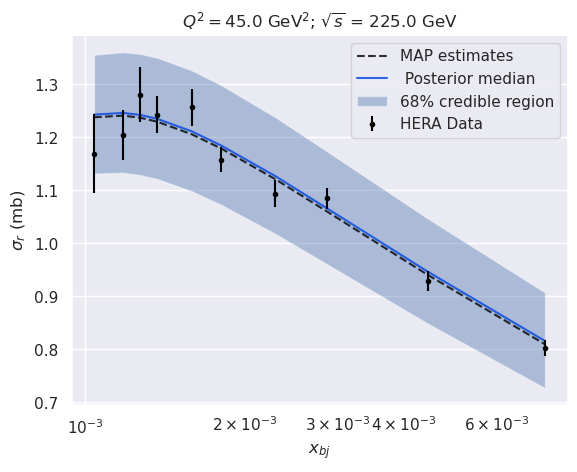
\includegraphics[width=0.5\textwidth]{figs\mve_map_vs_median_45_225.png}
\caption{MAP vs median at Q2 = 45.0 GeV and sqrt(s) = 225.0 GeV}
\label{fig:mve_map_vs_median_45_225}
\end{figure}

Here we have smaller Q2 = 8.5 GeV and sqrt(s) = 251.0 GeV.

\begin{figure}
\centering
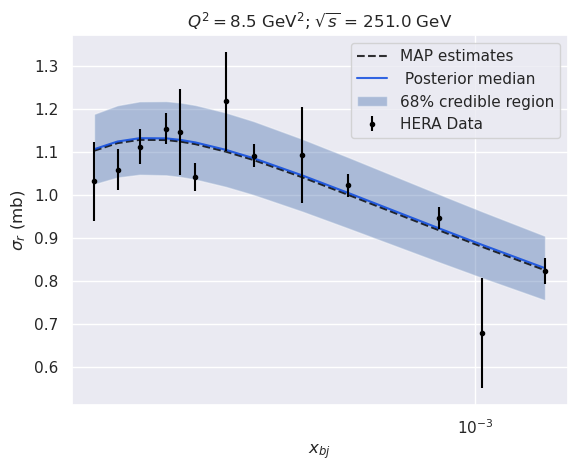
\includegraphics[width=0.5\textwidth]{figs\mve_map_vs_median_8pt5_251.png}
\caption{MAP vs median at Q2 = 8.5 GeV and sqrt(s) = 251.0 GeV}
\label{fig:mve_map_vs_median_8pt5_251}
\end{figure}

\section{2D Fourier Transform of Dipole Amplitude}

Now that we are confident with the parameters obtained from the MVe parametrization of the initial BK, we calculate the 2D Fourier Transform of Dipole scattering amplitude to obtain its dependence on dipole momentum, k. Below we have the plot with the 90\% confidence interval around the median, calculated for all posterior samples. The median curve is calculated by obtaining the median of all the S curves. We also normalize to 1 to see the behavior of the 2 sigma bands. We also graph the $\tilde{S}(k) * \sigma_0$ to see if it increases the uncertainty at $k \approx 0.5$.

\begin{figure}
\centering
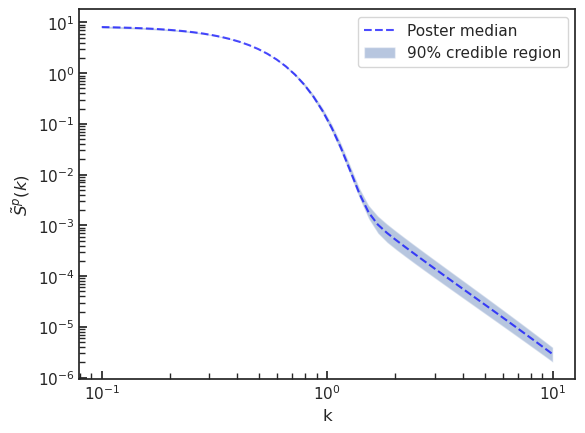
\includegraphics[width=0.5\textwidth]{figs\2dft.png}
\caption{2D Fourier Transform of Dipole Amplitude for $\tilde{S}(k)$ and for $\tilde{S}(k) * \sigma_0/2$}
\label{fig:2dft}
\end{figure}

This quantity is directly proportional to the $\gamma^{*} p$ cross section and from here we are able to calculate some observables.


\section{MV⁵}
Next thing we want to do is parametrize the initial condition of the rcBK model with 5 parameters, this time adding an extra parameter: the anomalous dimension gamma with bounds = [0.5, 2.0].

Plain LHS 

Quantiles:
[(0.05, 0.045782859856284594), (0.5, 0.05543492264182054), (0.95, 0.06661149569226865)]
Quantiles:
[(0.05, 1.3870639184518465), (0.5, 1.4301393304216496), (0.95, 1.4839272857686474)]
Quantiles:
[(0.05, 20.101847091178612), (0.5, 22.815519854142842), (0.95, 27.788593309639523)]
Quantiles:
[(0.05, 1.3684870673643048), (0.5, 13.985924494545358), (0.95, 36.06654216113256)]
Quantiles:
[(0.05, 16.251319717434143), (0.5, 17.249373723299552), (0.95, 18.368478185474505)]

$Q_{s0}^{2}$ (GeV²)= 0.057
$\gamma$= 1.436
$e_c$= 23.207
$C^{2}$= 15.936
$\sigma_0/2$ (mb)= 17.241
Mean acceptance fraction: 0.494

MAP estimates:  [ 0.05733286  1.42858461 22.66158827  0.47680259 17.12751157]
log posterior at MAP:  5.947365490438621
Median Values:  [ 0.05543492  1.43013933 22.81551985 13.98592449 17.24937372]
log posterior at Median:  5.458375051856651

\begin{figure}
\centering
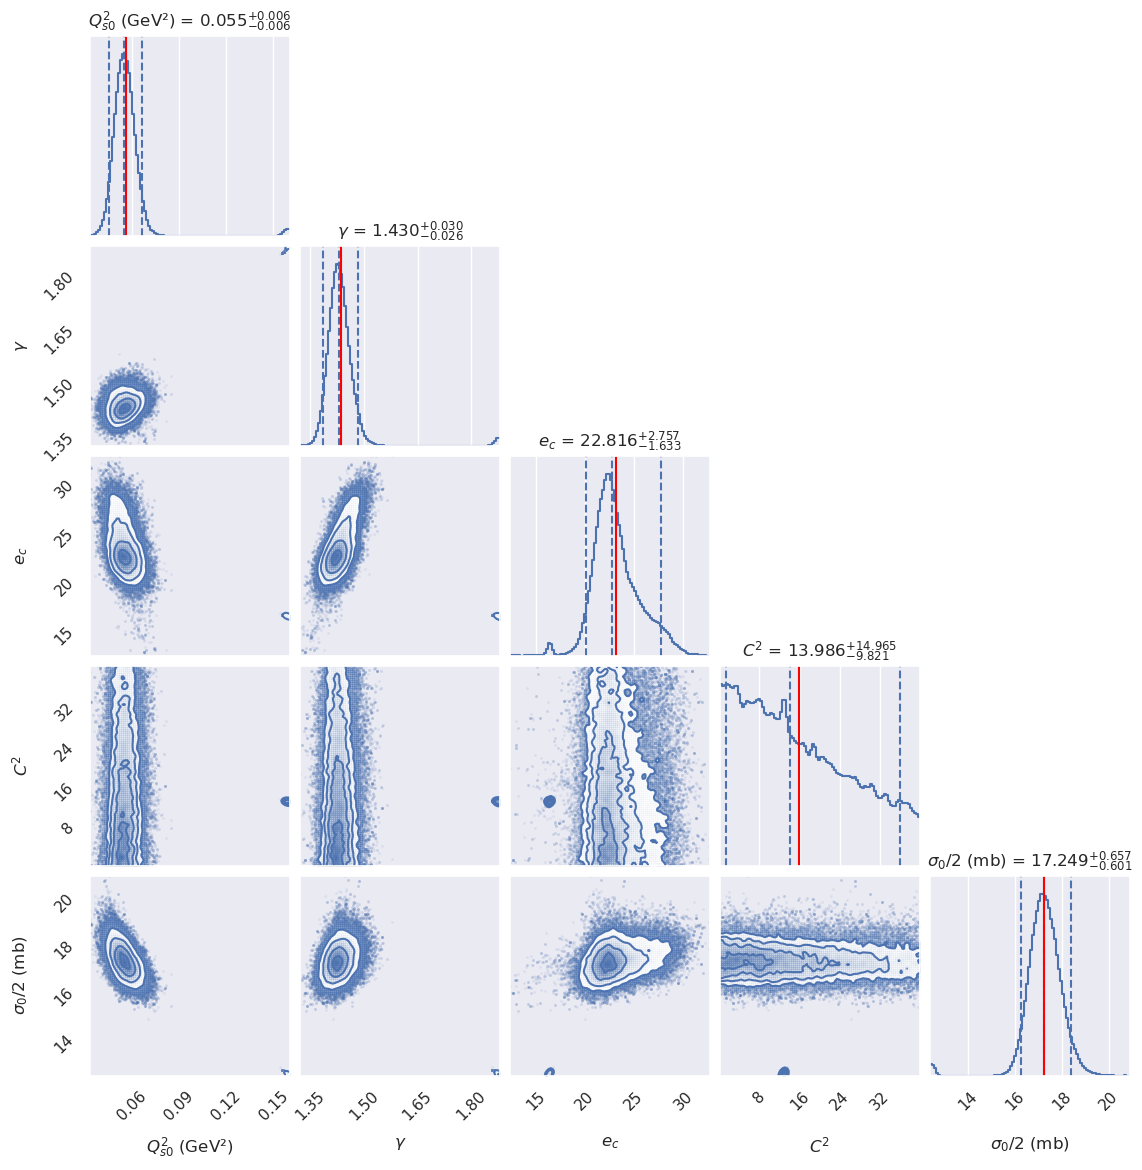
\includegraphics[width=0.5\textwidth]{figs\mv5_plainLHS_49d_100w_narrowinit.png}
\caption{Plain LHS for MV⁵ for 49 parameter samples and 100 walkers}
\label{fig:mv5_plainLHS_49d_100w_narrowinit}
\end{figure}

OrthLHS
Worse convergence has been observed with no special point in sight. We do not need to put all details here.

\begin{figure}
\centering
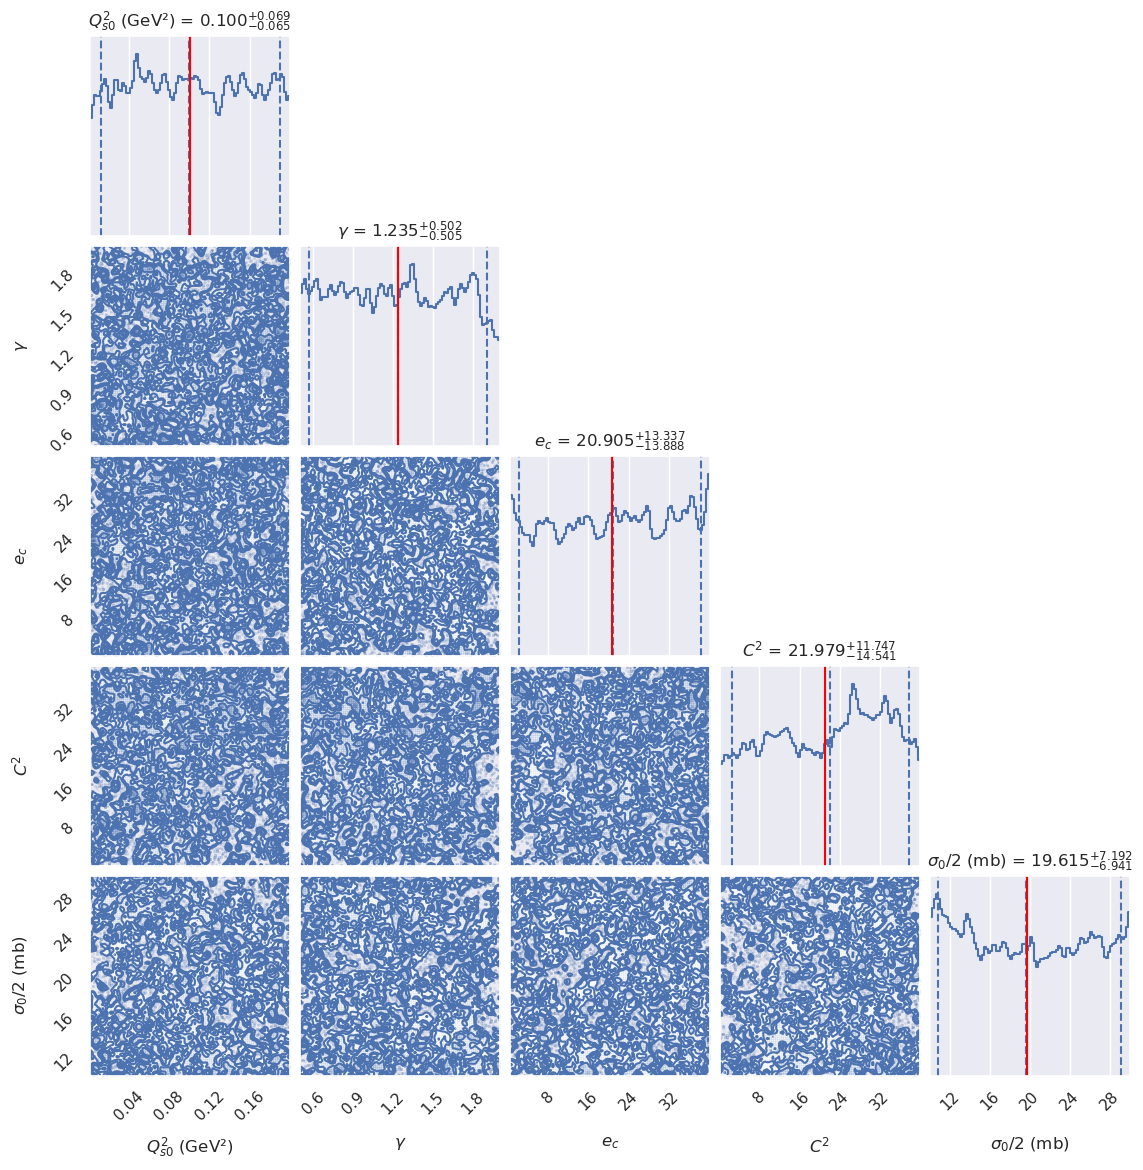
\includegraphics[width=0.5\textwidth]{figs\mv5_orthLHS_49d_50w_noburn.png}
\caption{Orthogonal LHS for MV⁵ for 49 parameter samples and 50 walkers}
\label{fig:mv5_orthLHS_49d_50w_noburn}
\end{figure}

Finally, we arrive at a convergence when we take 100 parameter samples. 

\begin{figure}
    \centering
    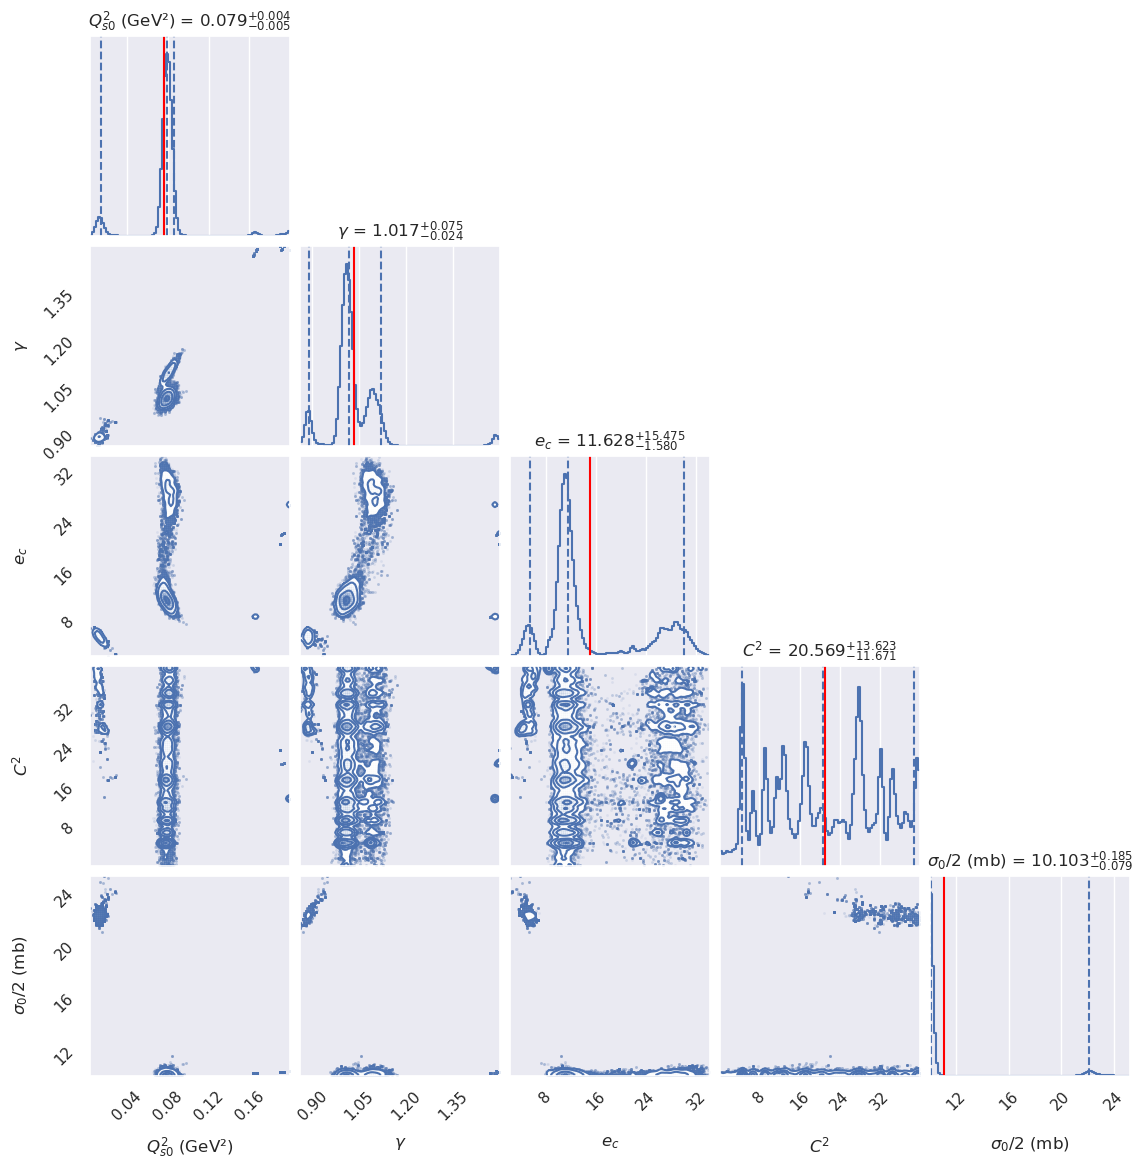
\includegraphics[width=0.5\textwidth]{figs\mv5_plainLHS_100d_100w.png}
    \caption{Plain LHS for MV⁵ for 100 parameter samples and 100 walkers initialized over the whole sampling space}
    \label{fig:mv5_plainLHS_100d_100w}
    \end{figure}

\subsection{Many Different Guesses}

The workflow of doing the emcee sampling is firstly initializing the walkers over the whole parameter space. This produces a posterior distribution that is peaked at particular positions in the parameter space but sometimes smallers peaks show. For this parametrization, the small peaks seam to be significant but much smaller than the main peak, anyway. 

\subsubsection{Median Initialization}
First and usual initialization technique we do is initialize the walkers over a small area around the median from the initial run. This produces a posterior distribution that is peaked at the same position as the initial run. This is what we want and usually we stop at this point.

\begin{figure}
\centering
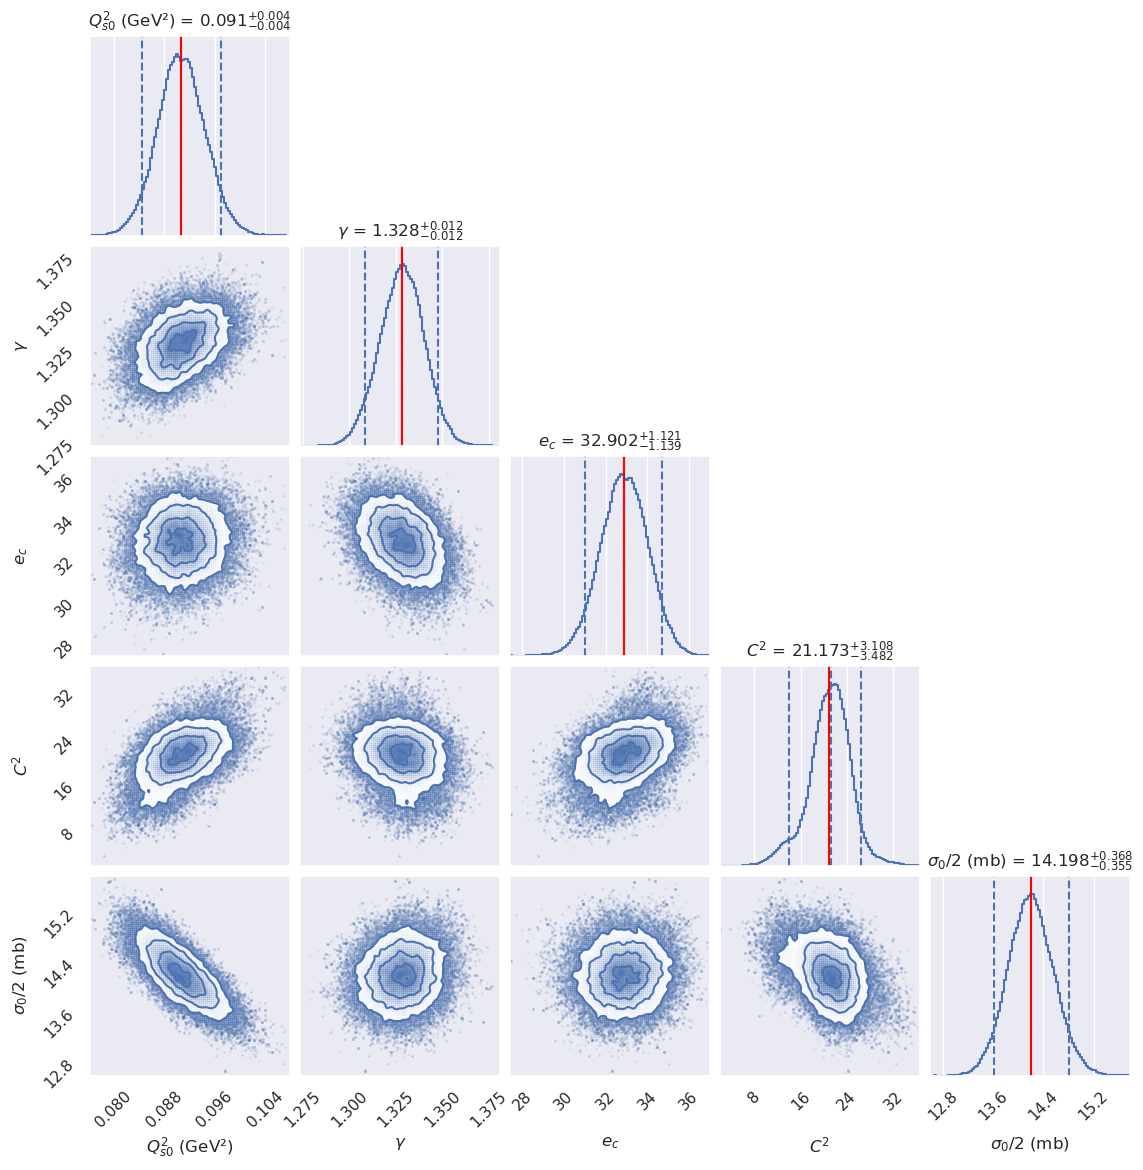
\includegraphics[width=0.5\textwidth]{figs\mv5_plainLHS_100d_widegamma_100w_narrowinit.png}
\caption{Plain LHS for MV⁵ for 100 parameter samples and 100 walkers initiazed around the median}
\end{figure}


\begin{figure}
\centering
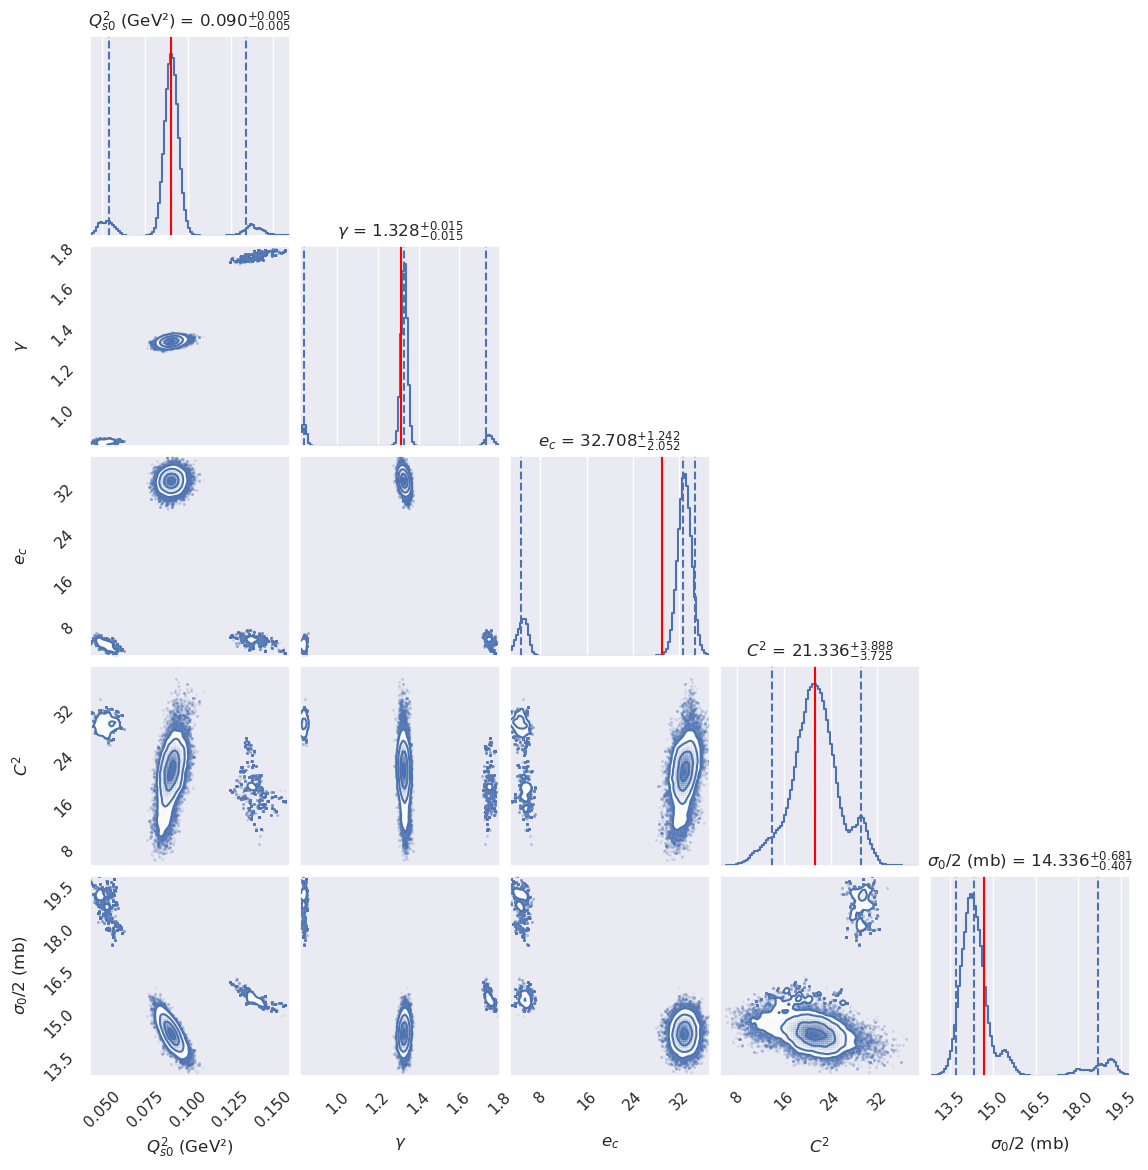
\includegraphics[width=0.5\textwidth]{figs\mv5_plainLHS_100d_widegamma_100w.png}
\caption{Plain LHS for MV⁵ for 100 parameter samples and 100 walkers}
\label{fig:mv5_plainLHS_100d_widegamma_100w}
\end{figure}
    
\begin{figure}
\centering
\includegraphics[width=0.5\textwidth]{figs\mv5_plainLHS_100d_widegamma_100w_chain.png}
\caption{Plain LHS for MV⁵ for 100 parameter samples and 100 walkers}
\label{fig:mv5_plainLHS_100d_widegamma_100w_chain}
\end{figure}
    
Details
Initialized over l_bounds_in = [0.08, 1.2, 30.0, 20.0, 13.0] and u_bounds_in = [0.10, 1.4, 35.0, 22.0, 15.0] centered around the peaks in the initial run. The results that we get 

$Q_{s0}^{2}$ (GeV²)= 0.091
$\gamma$= 1.328
$e_c$= 32.891
$C^{2}$= 20.953
$\sigma_0/2$ (mb)= 14.203
Mean acceptance fraction: 0.554

MAP estimates:  [ 0.09073768  1.32758085 32.94110629 21.20867231 14.19780092]
log posterior at MAP:  276.9905911240538
Median Values:  [ 0.09068555  1.32842287 32.90234842 21.17309616 14.19753749]
log posterior at Median:  276.9563399862609

\subsubsection{MVe Initialization}

However, we notice something weird happening where if we initialize the walkers in the a different gamma region using the values obtained in our mve run (gamma = 1) but we initialize C² over all space, we notice a convergence in different areas of the parameter space. This is not what we want. We want to have a convergence in the same region of the parameter space independent of the area of initialization. Does this suggest a multimodal posterior for gamma when left as a free parameter?

Let's examine.

\begin{figure}
\centering
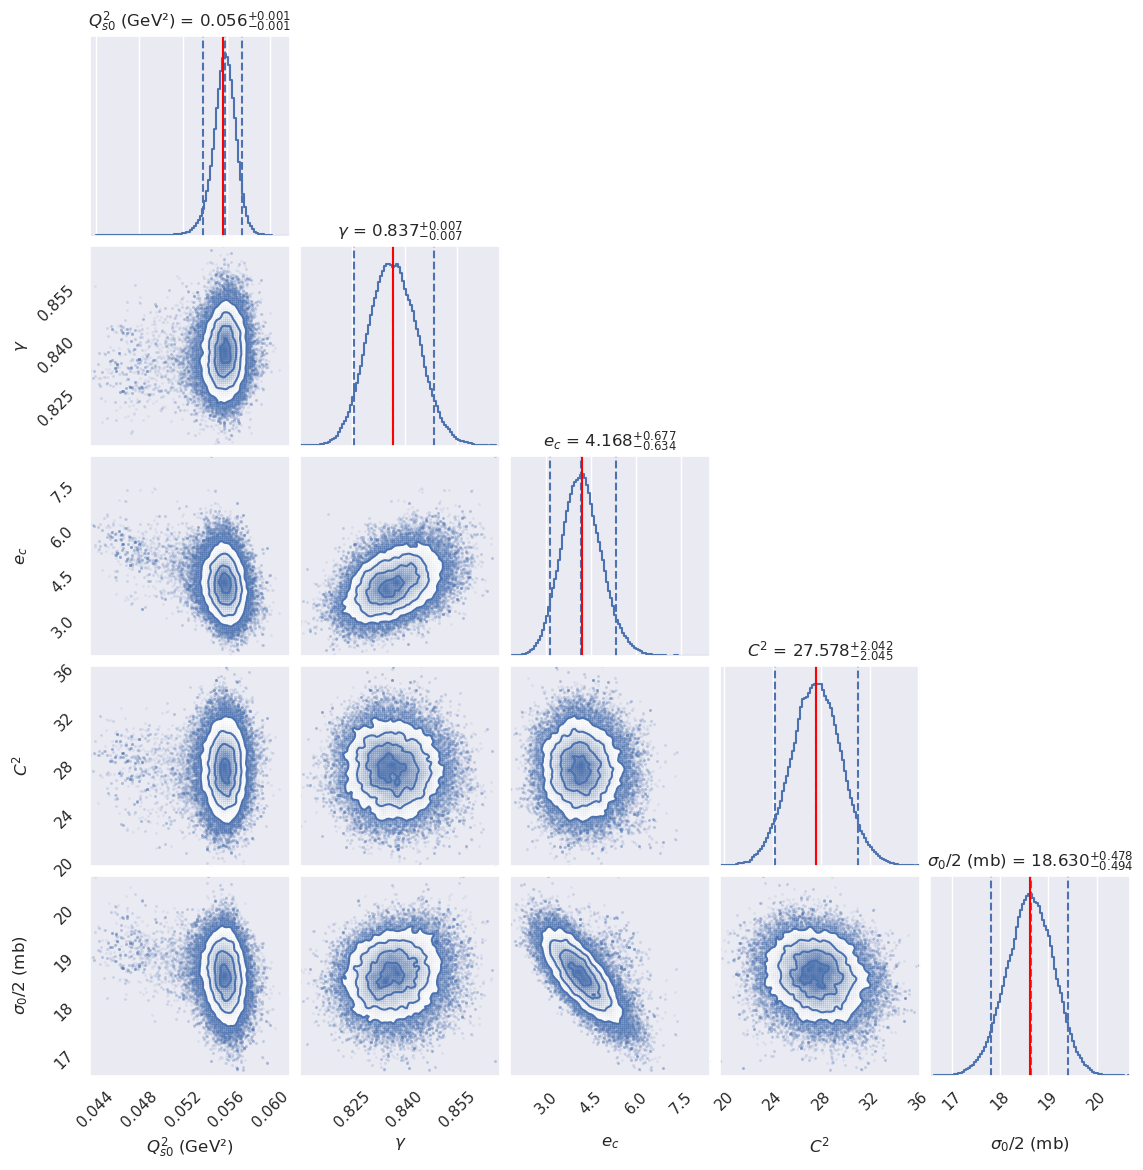
\includegraphics[width=0.5\textwidth]{figs\mv5_plainLHS_100d_widegamma_100w_mveinit.png}
\caption{Plain LHS for MV⁵ for 100 parameter samples and 100 walkers initiazed around the MVe MAP/median values}
\label{fig:mv5_plainLHS_100d_widegamma_100w_mveinit}
\end{figure}

The results are not converged in C².


\subsubsection{MAP Initialization}
We try a new technique by obtaining the MAP first with initial guess of gamma equal to that obtain in the rcbk paper. We use two different algorithms: minimize and basinhopping. We obtian the results here for the wide gamma range.

Initial Guess for minimize:  [ 0.06  1.   18.9   7.2  16.36]
minimize estimates:  [ 0.10165458  1.32284799 30.40428667  7.19999575 12.69743765]
log posterior at minimize -307.8329182008889
basinhopping estimates:  [ 0.10179309  1.32219056 30.50792323  6.2602836  12.68127956]
log posterior at basinhopping -307.837620177625

As predicted, the basinhopping does find a position where the negative of the log posterior is more minimized. The scipy.minimize has tendencies of finding local maxima around the initial guess, although this is okay for doing after finding the posteriors, it does not work in finding the global maxima of the posterior to initialize where the walkers are. 

This way of initializing walkers is documented in the emcee documentation: https://readthedocs.org/projects/emcee/downloads/pdf/v2.2.1/.

Unfortunately this does not work in converging all the parameters. 

\begin{figure}
\centering
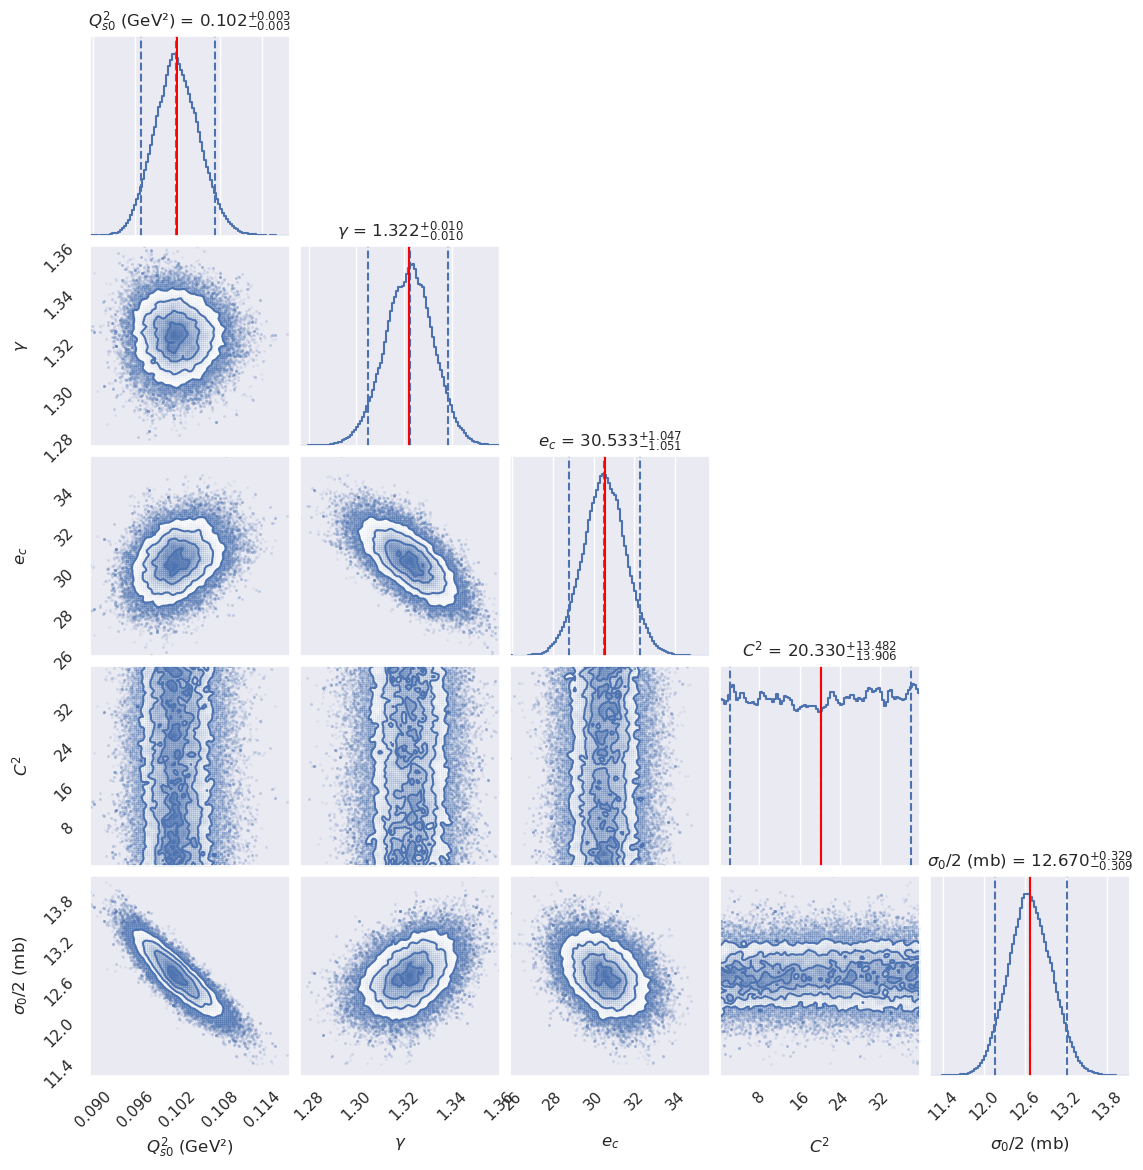
\includegraphics[width=0.5\textwidth]{figs\mv5_plainLHS_100d_widegamma_100w_mapinit.png}
\caption{Plain LHS for MV⁵ for 100 parameter samples and 100 walkers initiazed around initial MAP values}
\end{figure}


Here we do a different initial guess for the optimize function.
Initial Guess for minimize:  [ 0.07696357  1.          7.46144896  5.00327994 15.02871265]
minimize estimates:  [ 0.07415565  0.84142315  0.58291575  5.00327994 17.92891779]
log posterior at minimize -321.8459870643879
basinhopping estimates:  [ 0.06515335  0.84548206  0.50806373  4.93496011 20.08486134]
log posterior at basinhopping -326.35924880524703


\subsection{Narrow Gamma Range}

Oddly enough, the narrow gamma doesnot give proper convergence to other parameters. The MAP iinitialization:

Initial Guess for minimize:  y supporting documents you’ve brought with you.

[ 0.06  1.   18.9   7.2  16.36]
minimize estimates:  [1.07561115e-03 8.42458262e-01 1.45164097e+01 7.97672770e+00  1.58412078e+01]
log posterior at minimize -278.27712184232774
basinhopping estimates:  [ 0.08242398  1.09395535 27.26378182 12.25817616 10.03228508]
log posterior at basinhopping -338.53583454394544

Sadly, it does not help in the convergence of the other parameters.

\begin{figure}
\centering
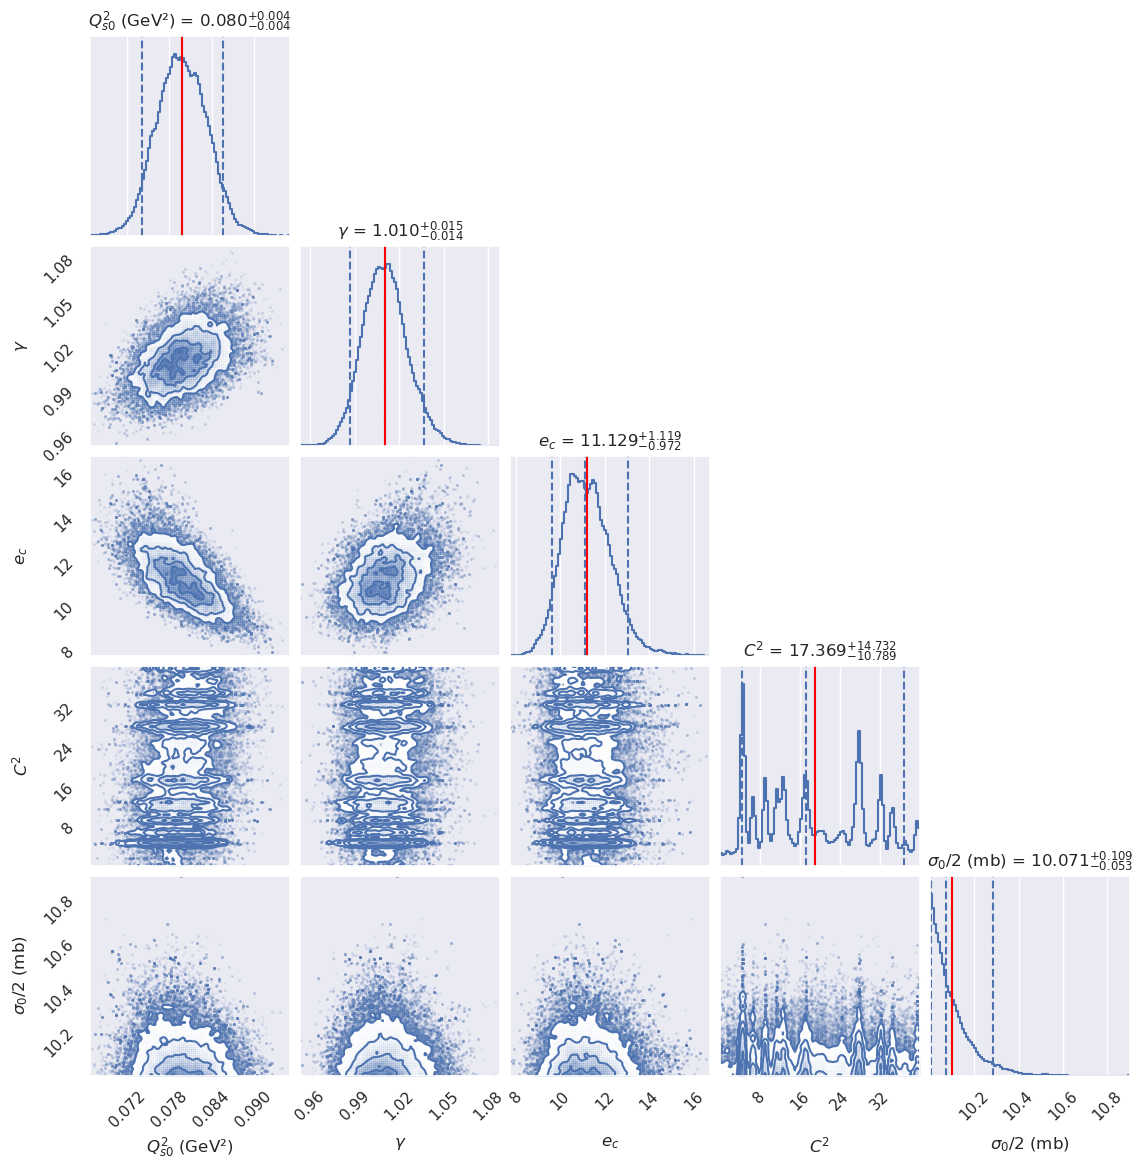
\includegraphics[width=0.5\textwidth]{figs\mv5_plainLHS_100d_100w_narrowinit.png}
\end{figure}

\subsection{Mistake correction: Qs02 range}
Mistake! We have been generating our parameter samples in a wide range of Qs02. Which was my mistake but it does not diminish the fact that our sampling is converging at different spots in the paramter space. The following results will now involve a Qs02 range that is from 0.001 to 2.0. More details: 20\% test values and 5 principal components.

Here is a figure of the posterior distribution if we use different moves (choice is completely random and is the shortest implementation we can make besides the default stretch move). 

\begin{figure}
\centering
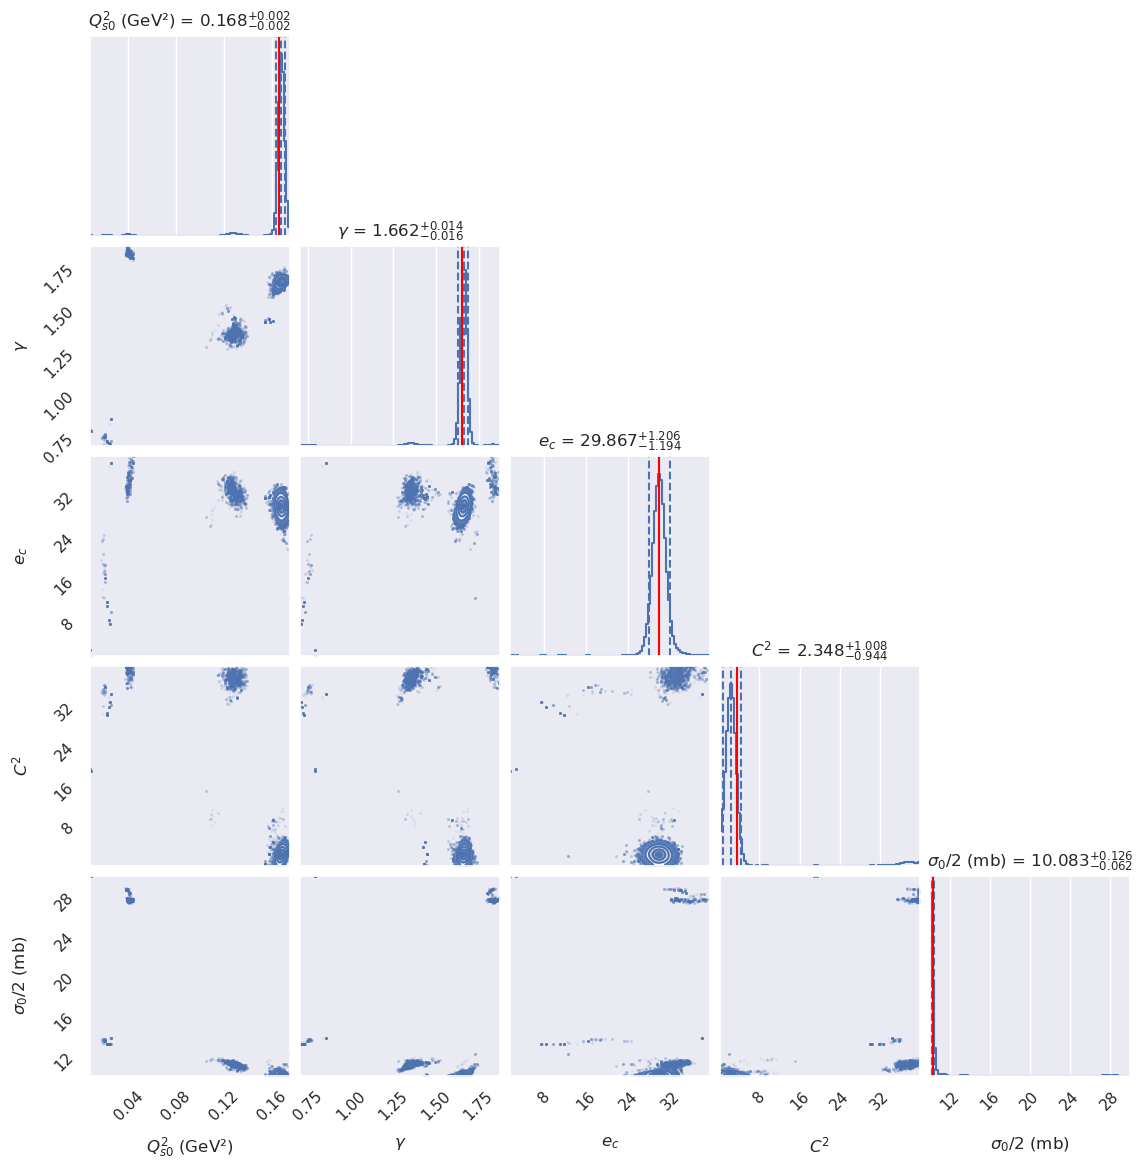
\includegraphics[width=0.5\textwidth]{figs\mv5_plainLHS_100d_corr_100w_DEMovecomb.png}
\caption(Plain LHS for the correct Qs02 range for 100 walkers and 100 parameter samples emcee using DEMove and DEsnookermove combination as walker move)
\label{fig:mv5_plainLHS_100d_corr_100w_DEMovecomb}
\end{figure}

These peaks, without bias initialization, actually match the basinhopping estimates. 
Initial Guess for minimize:  [ 0.07696357  1.          7.46144896  5.00327994 15.02871265]
minimize estimates:  [ 0.04146776  0.94703643 17.52542191 13.71100446 10.02567683]
log posterior at minimize -142.29413839385722
basinhopping estimates:  [ 0.16870158  1.65652093 29.52744335  2.51967912 10.01630848]
log posterior at basinhopping -396.51418335627807

We have definitely found peaks. Problem is these values are the edges of our space. We also have these values

$Q_{s0}^{2}$ (GeV²)= 0.166
$\gamma$= 1.653
$e_c$= 29.871
$C^{2}$= 3.492
$\sigma_0/2$ (mb)= 10.273
Mean acceptance fraction: 0.218


\subsection{Conclusion}

Let's try it again for more training samples. It is clear that the log posteriors for these multiple solutions are so close to each other (300 to 400) that the emcee sampling is considering both of them as valid solutions. Also we realize that different initializations give different median values which something we do not trust. If we were to decrease our Qs0_2 range, we would count on a better convergence. Walkers are stuck in islands of local maxima. 

\begin{figure}
\centering
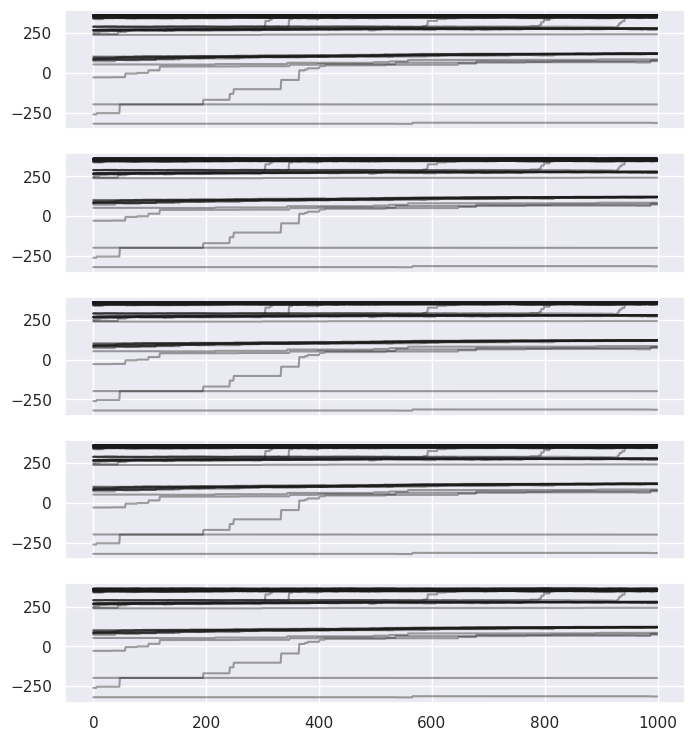
\includegraphics[width=0.5\textwidth]{figs\walkersinislands.png}'
\caption{Walkers in islands of local maxima}
\end{figure}


\subsection{150 Plain LHS}
We generate 150 parameter samples within bounds: 	
l_bounds = [.001, 0.5, .5, 0.1, 10.]
u_bounds = [0.2, 2.0, 40., 40., 30.]

We emcee sample, using a combination of DEMove and DEsnookermove over the whole parameter space and with more burn walks (2000) and 1000 walk samples, we find this final distribution that seem to have converged at two log posterior values. 

\begin{figure}
\centering
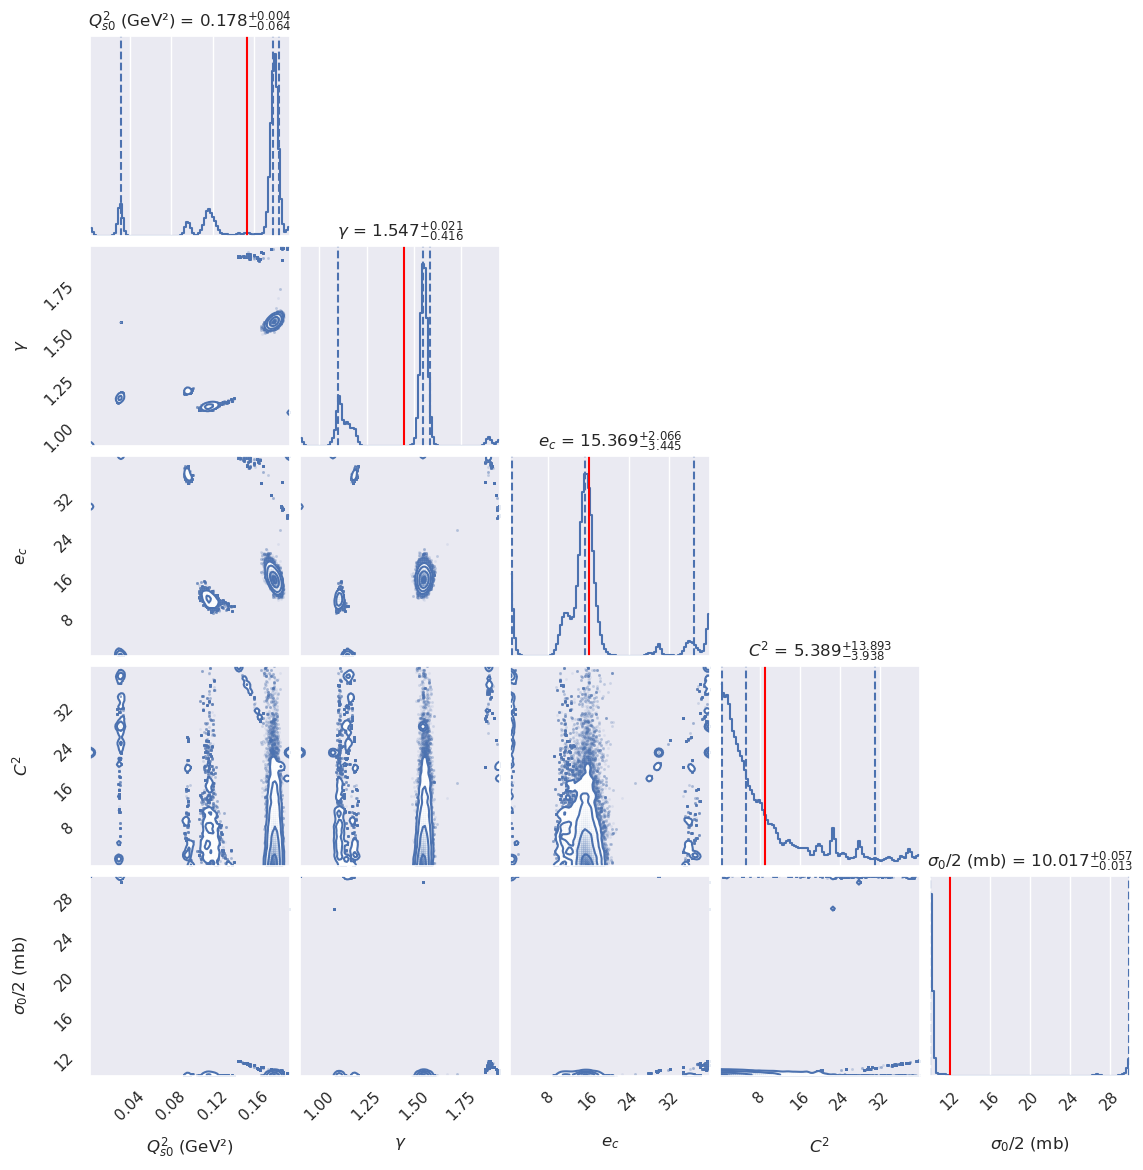
\includegraphics[width=0.5\textwidth]{figs\mv5_plainLHS_150d_100w_morewalks.png}
\caption{Plain LHS for 150 parameter samples and 100 walkers using a combination of DEMove and DEsnookermove}
\end{figure}

They seem to converge at two log posterior values. I guess because we are using a move combination meant for multimodal distributions, it might be more multimodal friendly hence the two peaks. If we swith to the default stretch move with still this much walkers, maybe we can get a better single peak. 

\begin{figure}
\centering
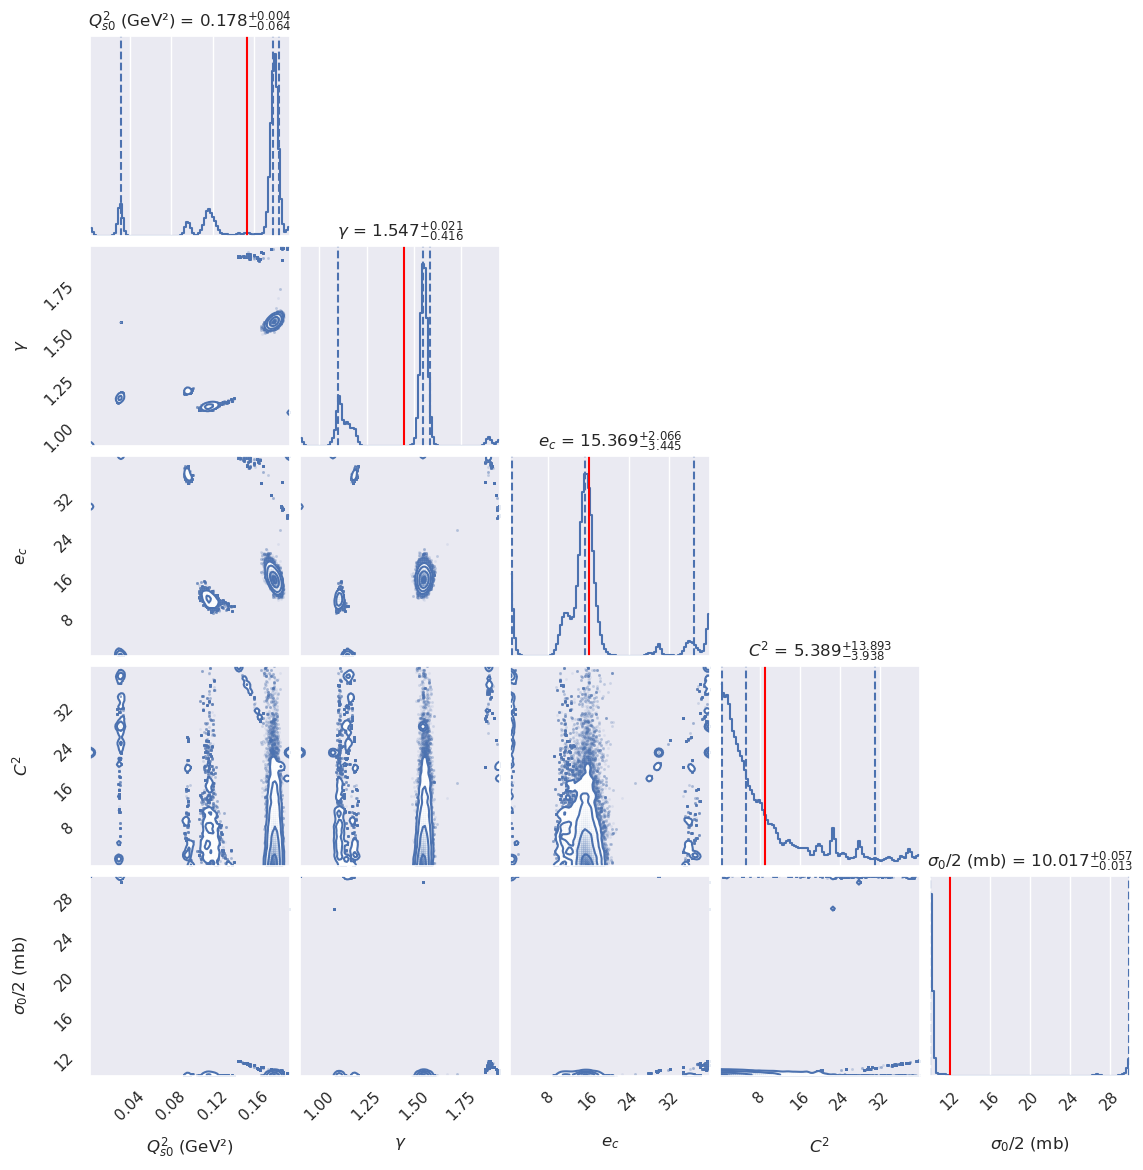
\includegraphics[width=0.5\textwidth]{figs\mv5_plainLHS_150d_100w_morewalks.png}
\caption{Plain LHS for 150 parameter samples and 100 walkers using a default stretch move}
\end{figure}

However we already see a pattern here. That the the paramter value for sigma0/2 skews toward the lower bound 10.0 mb. This might be consistent with the prescription for $$ \sigma_0 = 4\pi B_D $$ where $B_D \approx 4$ GeV giving $ \sigma_0 = 19.5 $ mb.

In both cases, we see that there are 2 or more peaks usually present. We wonder if there is a possibility that the log posterior is multimodal; however, one is has log probability higher than the other. 

Peak 1

l_bounds_in = [0.16, 1.0, 10.0, 4.0, 10.0] 
u_bounds_in = [0.19, 1.2, 12.0, 6.0, 14.0]
$Q_{s0}^{2}$ (GeV²)= 0.122
$\gamma$= 1.132
$e_c$= 11.482
$C^{2}$= 7.786
$\sigma_0/2$ (mb)= 10.020
Mean acceptance fraction: 0.419

MAP peak near median values: [ 0.1177862   1.10460418 11.45378404  5.6573639  10.01140716]
log posterior at MAP -355.80632170516776

Peak 2

$Q_{s0}^{2}$ (GeV²)= 0.178
$\gamma$= 1.543
$e_c$= 15.730
$C^{2}$= 5.906
$\sigma_0/2$ (mb)= 10.018
Mean acceptance fraction: 0.459

MAP peak near median values: [ 0.17985022  1.5528701  15.61781138  4.17604652 10.01358633]
log posterior at MAP -332.620602059257

Peak 3: initialized at 
l_bounds_in = [0.05, 0.75, 3.0, 24.0, 17.0]
u_bounds_in = [0.07, 0.90, 6.0, 32.0, 20.0]
from the mve peak in the first mv5 run

$Q_{s0}^{2}$ (GeV²)= 0.112
$\gamma$= 1.130
$e_c$= 11.795
$C^{2}$= 7.944
$\sigma_0/2$ (mb)= 11.218
Mean acceptance fraction: 0.365

MAP peak near median values: [ 0.11594505  1.10091539 11.50380359  5.69849215 10.00481906]
log posterior at MAP -356.0391175944104


Peak 4: initialized at
l_bounds_in = [0.08, 1.30, 30.0, 16.0, 13.0]
u_bounds_in = [0.10, 1.35, 36.0, 24.0, 15.0]
from the narrow initialization peak at the first mv5 runs

MAP peak near median values: [ 0.17978322  1.5515433  15.61865206  4.93474362 10.0004294 ]
log posterior at MAP -333.23268041177596

\subsection{5 to 30 sigma0}



\end{document}